\section{Hiện thực hệ thống}

\subsection{Cấu trúc mã nguồn}
Hệ thống được tổ chức theo mô hình monorepo, trong đó backend và frontend được tách thành hai workspace độc lập để thuận lợi cho phát triển song song và triển khai riêng vòng đời build/deploy.

\subsubsection{Tổ chức thư mục tổng thể}
Ở mức repository, mã nguồn được chia thành các khối chính:
\begin{itemize}
	\item \textbf{backend/}: mã nguồn NestJS, mô hình dữ liệu, module nghiệp vụ, scripts migration/seed.
	\item \textbf{frontend/}: mã nguồn React + TypeScript + Vite, các feature UI, i18n, utils.
	\item \textbf{grafana/, prometheus*.yml}: cấu hình giám sát vận hành.
	\item \textbf{docker-compose*.yml}: cấu hình môi trường chạy nhiều dịch vụ.
	\item \textbf{report/LuanVan/}: tài liệu luận văn và hình minh họa.
\end{itemize}

Việc tách các khối theo vai trò giúp quy trình cộng tác rõ ràng: nhóm backend tập trung logic nghiệp vụ và dữ liệu, nhóm frontend tập trung trải nghiệm người dùng, nhóm vận hành tập trung hạ tầng và quan sát hệ thống.

\subsubsection{Cấu trúc backend}
Backend được xây dựng trên NestJS và tổ chức theo module nghiệp vụ. Mỗi module thường gồm:
\begin{itemize}
	\item \texttt{controller}: định nghĩa endpoint và hợp đồng API.
	\item \texttt{service}: hiện thực logic nghiệp vụ và orchestration.
	\item \texttt{dto}: định nghĩa input/output contract và validation.
	\item \texttt{entity}: ánh xạ bảng dữ liệu qua TypeORM.
\end{itemize}

Các module lõi đã triển khai gồm xác thực/ủy quyền, người dùng, tổ chức, CTXH, thu phí, biểu mẫu, chatbot RAG, cấu hình S3, xuất báo cáo và quan sát metrics.

Luồng xử lý chuẩn trong backend:
\begin{enumerate}
	\item Request đi vào controller.
	\item Guard và pipe kiểm tra xác thực, quyền hạn, định dạng dữ liệu.
	\item Service xử lý nghiệp vụ và gọi repository/entity.
	\item Kết quả trả về dạng JSON chuẩn hóa cho frontend.
\end{enumerate}

\subsubsection{Cấu trúc frontend}
Frontend sử dụng React + Vite + TypeScript. Cấu trúc mã nguồn được tổ chức theo feature để bám sát nghiệp vụ:
\begin{itemize}
	\item \textbf{features/}: các phân hệ như người dùng, tổ chức, CTXH, payment, template, chatbot.
	\item \textbf{shared/}: component dùng chung, constants, hooks và kiểu dữ liệu dùng lại.
	\item \textbf{i18n/}: cấu hình đa ngôn ngữ và tài nguyên dịch.
	\item \textbf{utils/}: tiện ích xử lý dữ liệu phía client.
\end{itemize}

Frontend giao tiếp backend qua \texttt{axios} và quản lý vòng đời truy vấn bằng \texttt{React Query}. Cách tổ chức này giúp dữ liệu đồng bộ tốt giữa các màn hình, giảm gọi API dư thừa và kiểm soát rõ trạng thái loading/error.

\subsection{Các module và API chính}

\subsubsection{Module xác thực và phân quyền}
Module xác thực hiện thực các chức năng đăng nhập nội bộ, đăng nhập Google OAuth, refresh token, logout, lấy profile và lấy quyền hiện tại của người dùng.

Các endpoint điển hình:
\begin{itemize}
	\item \texttt{POST /auth/login}
	\item \texttt{POST /auth/refresh}
	\item \texttt{POST /auth/logout}
	\item \texttt{GET /auth/profile}
	\item \texttt{GET /auth/me/permissions}
	\item \texttt{GET /auth/google}, \texttt{GET /auth/google/callback}
\end{itemize}

Sau xác thực, hệ thống áp dụng RBAC theo ngữ cảnh tổ chức. Người dùng có thể được cấp nhiều vai trò trên nhiều đơn vị khác nhau. Khi frontend gọi API nghiệp vụ, guard phân quyền sẽ đối chiếu quyền yêu cầu với bộ quyền hiệu lực của người dùng tại scope tương ứng.

\subsubsection{Module quản lý người dùng, tổ chức, khoa, lớp}
Các module quản trị dữ liệu nền hiện thực đầy đủ CRUD, phân trang, lọc, import/export Excel và một số luồng batch processing cho dữ liệu lớn.

\textbf{Người dùng:}
\begin{itemize}
	\item \texttt{GET /users}, \texttt{GET /users/:id}, \texttt{POST /users}, \texttt{PATCH /users/:id}, \texttt{DELETE /users/:id}
	\item \texttt{POST /users/import/upload}
	\item \texttt{GET /users/import/:sessionId/validate}
	\item \texttt{POST /users/import/:sessionId/execute}
	\item \texttt{POST /users/import/batch} cho kịch bản import phía client theo lô lớn
\end{itemize}

\textbf{Tổ chức:}
\begin{itemize}
	\item \texttt{GET /organizations/tree}, \texttt{GET /organizations/:id/children}
	\item \texttt{GET /organizations/stats}, \texttt{GET /organizations/accessible}
	\item Các endpoint tối ưu truy vấn theo độ sâu cây và theo loại/mã tổ chức
\end{itemize}

\textbf{Khoa/Lớp:}
\begin{itemize}
	\item CRUD chuẩn cho \texttt{/departments} và \texttt{/classes}
	\item Hỗ trợ import theo session và import batch
\end{itemize}

\subsubsection{Module CTXH}
Module CTXH bao gồm quản lý danh mục, hoạt động, người tham gia, cấu hình giới hạn và báo cáo:
\begin{itemize}
	\item \texttt{/ctxh/categories}: tạo/sửa/xóa/xem danh mục phân loại hoạt động CTXH.
	\item \texttt{/ctxh/activities}: tạo/sửa/xóa/lọc hoạt động theo trạng thái, thời gian, tổ chức, danh mục.
	\item \texttt{/ctxh/limit-config}: quản lý cấu hình số ngày CTXH tối đa theo tổ chức.
	\item \texttt{/ctxh/import/old-system}: validate và nhập dữ liệu CTXH từ hệ thống cũ.
	\item \texttt{/ctxh/reports/student/:studentCode}: báo cáo CTXH cá nhân theo MSSV.
\end{itemize}

Các luồng import/chấm điểm được thiết kế theo hướng chịu tải file lớn, có bước validate trước khi commit để giảm rủi ro lỗi dữ liệu hàng loạt.

\subsubsection{Module thu phí}
Module thu phí hiện thực theo mô hình campaign-based:
\begin{itemize}
	\item \texttt{/payment-campaigns}: quản lý chiến dịch thu phí và vòng đời trạng thái.
	\item \texttt{/payment-fee-levels}: quản lý mức phí trong từng campaign.
	\item \texttt{/payment/assignments}: gán nghĩa vụ đóng phí cho người dùng, theo dõi trạng thái pending/paid/overdue.
	\item \texttt{/payment-campaigns/:id/payos-config}: cấu hình PayOS theo campaign.
	\item \texttt{/api/payment-admin/*}: các endpoint kiểm tra/sync dữ liệu giao dịch phục vụ vận hành.
\end{itemize}

Thiết kế này tách rõ: cấu hình nghiệp vụ (campaign/fee), phân công đối tượng (assignment), và lịch sử giao dịch thực tế (payment history), giúp đối soát dễ dàng và truy xuất đầy đủ audit trail.

\subsubsection{Module biểu mẫu điện tử}
Module biểu mẫu gồm hai phần chính:
\begin{itemize}
	\item \texttt{/templates}: upload template Word, parse placeholder, cấu hình field động.
	\item \texttt{/submissions}: lưu draft, submit, sinh tài liệu đầu ra, tải file và lấy public URL.
\end{itemize}

Quy trình hiện thực:
\begin{enumerate}
	\item Quản trị viên upload \texttt{.docx}.
	\item Hệ thống parse placeholder và sinh schema field.
	\item Người dùng điền biểu mẫu động.
	\item Backend render file Word, lưu file lên S3 và lưu metadata vào database.
\end{enumerate}

\subsubsection{Bảng tổng hợp API chính theo module}
Để thuận tiện theo dõi ở góc độ triển khai, bảng sau tổng hợp các nhóm API đại diện đang vận hành trong hệ thống.

\begin{table}[H]
\centering
\renewcommand{\arraystretch}{1.2}
\small
\begin{tabular}{|p{3.2cm}|p{5.5cm}|p{6.3cm}|}
\hline
\textbf{Module} & \textbf{Nhóm endpoint chính} & \textbf{Mục đích nghiệp vụ} \\
\hline
Auth \& RBAC & \texttt{/auth/*}, \texttt{/roles/*} & Xác thực, quản lý phiên, lấy quyền và phân vai trò theo ngữ cảnh tổ chức \\
\hline
Users & \texttt{/users/*}, \texttt{/users/import/*} & Quản lý người dùng, import dữ liệu lớn, gán vai trò và lọc danh sách \\
\hline
Organizations & \texttt{/organizations/*} & Quản lý cây tổ chức, tra cứu theo cấp, thống kê và quyền truy cập theo user \\
\hline
Classes/Departments & \texttt{/classes/*}, \texttt{/departments/*} & Quản lý dữ liệu học thuật nền và import batch \\
\hline
CTXH & \texttt{/ctxh/activities/*}, \texttt{/ctxh/limit-config/*}, \texttt{/ctxh/reports/*} & Vận hành vòng đời hoạt động, chấm điểm, giới hạn ngày và báo cáo \\
\hline
Payment & \texttt{/payment-campaigns/*}, \texttt{/payment/assignments/*}, \texttt{/api/payment-admin/*} & Quản lý chiến dịch thu phí, phân công đóng phí, đối soát và vận hành giao dịch \\
\hline
Templates & \texttt{/templates/*}, \texttt{/submissions/*} & Upload template, cấu hình field động, nộp biểu mẫu và sinh tài liệu \\
\hline
RAG Chatbot & \texttt{/api/ctxh-chat/*} & Hỏi-đáp ngữ nghĩa, quản lý lịch sử hội thoại, ingestion và health check \\
\hline
Infra Support & \texttt{/aws-s3-config/*}, \texttt{/export/*} & Quản lý cấu hình lưu trữ và xuất dữ liệu nghiệp vụ \\
\hline
\end{tabular}
\caption{Tổng hợp API chính theo module}
\end{table}

\subsection{Hiện thực Chatbot CTXH}

\subsubsection{Mục tiêu hiện thực}
Chatbot được hiện thực để giải quyết bài toán tra cứu CTXH bằng ngôn ngữ tự nhiên trong bối cảnh dữ liệu hoạt động nhiều, thay đổi liên tục, và người dùng cần câu trả lời nhanh nhưng vẫn truy vết được nguồn. Đồng thời, hỗ trợ cán bộ trong công việc quản lý dữ liệu CTXH một cách nhanh chóng.

Các mục tiêu kỹ thuật chính:
\begin{itemize}
	\item Truy vấn ngữ nghĩa dựa trên dữ liệu nội bộ CTXH.
	\item Trả lời có nguồn trích dẫn.
	\item Hỗ trợ hội thoại nhiều lượt với session.
	\item Tối ưu cân bằng giữa độ đúng, độ phủ và chi phí vận hành.
\end{itemize}

\subsubsection{Kiến trúc kỹ thuật của module chatbot}
Module chatbot đặt trong namespace \texttt{ctxh-chat} ở backend và được tổ chức thành 17 service chuyên biệt, chia thành bốn lớp chức năng:

\textbf{Lớp điều phối (Orchestration):}
\begin{itemize}
	\item \textbf{LangChainRagChainService:} điều phối toàn bộ luồng 8 bước cho sinh viên: router agent, rewrite, truy xuất, enrichment, generation, follow-up.
	\item \textbf{StaffAgentService:} hiện thực vòng lặp ReAct tool-calling cho cán bộ, tối đa 10 vòng lặp, với 12 công cụ tuỳ chỉnh và các công cụ MCP.
\end{itemize}

\textbf{Lớp truy xuất và lưu trữ (Retrieval \& Storage):}
\begin{itemize}
	\item \textbf{LangChainVectorStoreService:} quản lý kết nối pgvector, cosine similarity search, MMR, metadata filters theo bộ điều kiện lọc.
	\item \textbf{CtxhFilterExtractionService:} dùng LLM để trích xuất bộ lọc có cấu trúc (thời gian, tổ chức, địa điểm, trạng thái) từ câu hỏi tự nhiên.
	\item \textbf{UserContextService:} tra cứu khoa đào tạo của sinh viên để thêm thông tin tổ chức của người dùng vào ngữ cảnh truy vấn.
	\item \textbf{McpMetadataEnricherService:} làm phong phú tài liệu truy xuất được bằng dữ liệu thời gian thực (số suất còn lại, yêu cầu duyệt).
	\item \textbf{McpSqlFallbackService:} truy vấn SQL dự phòng khi pgvector trả về 0 kết quả.
\end{itemize}

\textbf{Lớp MCP và giao tiếp ngoài (External Protocol):}
\begin{itemize}
	\item \textbf{PostgresMcpClientService:} wrapper quanh MCP SDK, giao tiếp với MCP server qua SSE để thực thi SQL trực tiếp.
	\item \textbf{FollowUpSuggestionsService:} sinh 3 câu gợi ý hội thoại tiếp theo sau mỗi lượt trả lời (timeout 4 giây).
\end{itemize}

\textbf{Lớp hạ tầng (Infrastructure):}
\begin{itemize}
	\item \textbf{LangChainMemoryService:} quản lý lịch sử hội thoại theo session (TTL 30 phút, tối đa 1000 session, 20 tin nhắn/session).
	\item \textbf{LangChainIngestionService:} thực thi pipeline embedding full/incremental vào bảng \texttt{ctxh\_embeddings}.
	\item \textbf{CtxhVectorSyncService:} nhận sự kiện từ TypeORM subscriber và đẩy job vào hàng đợi BullMQ.
	\item \textbf{VectorIngestionProcessor:} worker xử lý job embedding bất đồng bộ với chiến lược retry.
\end{itemize}

Thiết kế chia nhỏ service theo trách nhiệm đơn giúp dễ kiểm thử từng thành phần, đồng thời linh hoạt khi thay đổi mô hình LLM, embedding provider hoặc phương thức truy xuất.

\subsubsection{Dữ liệu đầu vào cho RAG và chuẩn hóa embedding}
Nguồn dữ liệu phục vụ chatbot lấy từ thực thể \texttt{CtxhActivity} với các quan hệ \texttt{organization} và \texttt{category} được load sẵn. Hàm \texttt{prepareDocuments()} chuyển đổi mỗi hoạt động thành một \texttt{Document} gồm hai phần tách biệt:

\textbf{Phần văn bản (\texttt{pageContent}) — dữ liệu được nhúng thành vector:}
\begin{itemize}
	\item \texttt{name}: tên hoạt động (tiền tố ``Hoạt động CTXH: ...'').
	\item \texttt{description}: mô tả hoạt động, mặc định là ``Không có mô tả'' nếu rỗng.
\end{itemize}

\textbf{Phần siêu dữ liệu (\texttt{metadata}) — dùng để lọc và truy xuất:}
\begin{itemize}
	\item \texttt{activityId}, \texttt{activityName}: định danh để liên kết kết quả tìm kiếm với bản ghi gốc.
	\item \texttt{organizationName}, \texttt{categoryName}: tên tổ chức chủ trì và danh mục CTXH.
	\item \texttt{startDate}, \texttt{endDate}: thời điểm bắt đầu/kết thúc (ISO~8601).
	\item \texttt{totalDays}: số ngày CTXH được ghi nhận.
	\item \texttt{location}: địa điểm tổ chức.
	\item \texttt{status}: trạng thái hoạt động (\texttt{ACTIVE}, \texttt{COMPLETED}, v.v.).
	\item \texttt{chunkType}: luôn là \texttt{full\_activity} — chiến lược chia chunk hiện tại là một chunk cho mỗi hoạt động.
\end{itemize}

Việc tách \texttt{pageContent} và \texttt{metadata} cho phép pgvector thực hiện tìm kiếm ngữ nghĩa trên nội dung văn bản trong khi vẫn lọc chính xác theo điều kiện cấu trúc (thời gian, tổ chức, trạng thái) mà không làm nhiễu không gian vector.

\subsubsection{Pipeline ingestion và đồng bộ vector}
Hệ thống hỗ trợ hai chế độ ingestion:
\begin{itemize}
	\item \textbf{Full ingestion:} tái tạo vector cho toàn bộ tập hoạt động.
	\item \textbf{Incremental ingestion:} chỉ cập nhật các bản ghi thay đổi theo mốc thời gian.
\end{itemize}

Quy trình ingestion gồm các bước:
\begin{enumerate}
	\item Đọc dữ liệu hoạt động và quan hệ liên quan.
	\item Chuẩn hóa text, tách chunk nếu cần.
	\item Tạo embedding theo provider cấu hình.
	\item Ghi vector + metadata vào bảng \texttt{ctxh\_embeddings}.
	\item Cập nhật chỉ mục và thống kê trạng thái ingestion.
\end{enumerate}

Thiết kế này cho phép khởi tạo nhanh dữ liệu AI khi triển khai mới và bảo trì linh hoạt trong vận hành định kỳ. Sequence diagram mô tả toàn bộ pipeline này được trình bày tại Hình~\ref{fig:seq-ingestion} (Mục~3.4.7).

\textbf{Tự động đồng bộ vector khi dữ liệu thay đổi:} Ngoài hai chế độ ingestion thủ công, hệ thống còn hiện thực cơ chế \textbf{auto-sync} theo kiến trúc hướng sự kiện. \texttt{CtxhActivitySubscriber} là TypeORM Entity Subscriber lắng nghe mọi thay đổi trên bảng \texttt{ctxh\_activity}:
\begin{itemize}
	\item \texttt{afterInsert}: hoạt động mới được tạo $\rightarrow$ đẩy job \texttt{UPSERT} vào hàng đợi.
	\item \texttt{afterUpdate}: hoạt động được cập nhật (nội dung, trạng thái, ngày, v.v.) $\rightarrow$ đẩy job \texttt{UPSERT} để embedding lại.
	\item \texttt{afterRemove}: hoạt động bị xóa $\rightarrow$ đẩy job \texttt{DELETE} để xóa vector tương ứng.
\end{itemize}

Các job được xử lý bất đồng bộ bởi \texttt{VectorIngestionProcessor} — một BullMQ worker với cấu hình: \texttt{concurrency=1} (đảm bảo thứ tự), 3 lần thử lại khi lỗi với thời gian chờ tăng dần theo cấp số nhân (2s $\rightarrow$ 4s $\rightarrow$ 8s). Cơ chế này đảm bảo dữ liệu trong vector store luôn phản ánh trạng thái mới nhất của database mà không cần can thiệp thủ công. Ngoài ra, một cron job chạy mỗi giờ thực hiện incremental sync như lớp dự phòng cuối để xử lý các trường hợp ngoại lệ (service restart, job thất bại vĩnh viễn).

\subsubsection{Kiến trúc Agentic và phân luồng theo vai trò người dùng}
Chatbot CTXH được thiết kế theo mô hình \textbf{agentic AI}, trong đó LLM không chỉ sinh văn bản mà còn tự quyết định gọi công cụ nào, theo thứ tự nào, dựa trên nội dung hội thoại và kết quả trả về từ từng công cụ. Kiến trúc này khác biệt căn bản so với mô hình RAG thụ động truyền thống, nơi hệ thống luôn thực hiện một quy trình cố định: truy xuất sau đó tổng hợp và sinh câu trả lời.

\textbf{Phân luồng theo vai trò:} Controller nhận request và xác định luồng xử lý dựa trên vai trò của người dùng xác thực qua JWT:

\begin{table}[H]
\centering
\renewcommand{\arraystretch}{1.3}
\begin{tabular}{|p{3.5cm}|p{5.5cm}|p{5.5cm}|}
\hline
\textbf{Tiêu chí} & \textbf{Sinh viên} & \textbf{Cán bộ} \\
\hline
Service xử lý & \texttt{LangChainRagChainService} & \texttt{StaffAgentService} \\
\hline
Mô hình xử lý & Router Agent + RAG pipeline & ReAct tool-calling \\
\hline
Số công cụ & 4 công cụ truy xuất & 12 công cụ CRUD + MCP tools \\
\hline
Khả năng ghi dữ liệu & Chỉ đọc + đăng ký hoạt động & Tạo/sửa/xóa hoạt động, duyệt đăng ký \\
\hline
Nguồn dữ liệu & pgvector (semantic search) & pgvector + SQL trực tiếp qua MCP \\
\hline
Context Injection & khoa đào tạo & danh sách hoạt động đang diễn ra \\
\hline
Gửi email & Không & Gửi email xác nhận duyệt/từ chối \\
\hline
\end{tabular}
\caption{So sánh luồng sinh viên và luồng cán bộ trong chatbot CTXH}
\end{table}

\textbf{Giới hạn tốc độ:} Cả hai luồng đều áp dụng rate limiting qua \texttt{RateLimitInterceptor} với Redis làm backend lưu trữ bộ đếm — mặc định 30 yêu cầu/60 giây/người dùng. Cơ chế này bảo vệ hệ thống khỏi quá tải do vòng lặp gọi API đồng thời.

\subsubsection{Pipeline trả lời câu hỏi}
Luồng xử lý truy vấn người dùng được hiện thực theo các pha sau:
\begin{enumerate}
	\item \textbf{Nhận request hội thoại:} API nhận \texttt{message}, \texttt{sessionId} và ngữ cảnh người dùng.
	\item \textbf{Tiền xử lý câu hỏi:} router xác định intent, rewrite câu hỏi nếu cần theo ngữ cảnh hội thoại.
	\item \textbf{Retrieval:} thực hiện tìm kiếm vector với chiến lược phù hợp (semantic/filter/MMR/multi-query).
	\item \textbf{Generation:} gửi context truy xuất được vào LLM để sinh câu trả lời tự nhiên.
	\item \textbf{Hậu xử lý:} chuẩn hóa output, gắn nguồn tham chiếu, ghi lịch sử hội thoại.
\end{enumerate}

Module hỗ trợ cả chế độ trả lời thường và stream SSE, phù hợp cho giao diện chat thời gian thực. Sequence diagram tổng thể của luồng này được mô tả tại Hình~\ref{fig:seq-student-rag} (Mục~3.4.7).

\subsubsection{Luồng sinh viên: Router Agent và phân loại ý định}
Bước đầu tiên trong luồng sinh viên là \textbf{Router Agent} — một lần gọi LLM có nhiệm vụ phân loại ý định câu hỏi và viết lại câu hỏi nếu cần. Router sử dụng prompt có cấu trúc kết hợp với lịch sử hội thoại để phân loại vào một trong bốn ý định:

\begin{table}[H]
\centering
\renewcommand{\arraystretch}{1.25}
\begin{tabular}{|p{3.8cm}|p{10.5cm}|}
\hline
\textbf{Ý định} & \textbf{Hành vi xử lý} \\
\hline
\texttt{RAG\_QUERY} & Thực hiện pipeline truy xuất và generation đầy đủ. \\
\hline
\texttt{REGISTER\_ACTIVITY} & Tìm hoạt động phù hợp, xác nhận với người dùng và thực hiện đăng ký tự động. \\
\hline
\texttt{GREETING} & Trả lời chào hỏi trực tiếp không cần truy xuất dữ liệu. \\
\hline
\texttt{CHITCHAT} & Xử lý trò chuyện thông thường không liên quan đến CTXH. \\
\hline
\end{tabular}
\caption{Phân loại ý định trong Router Agent của chatbot sinh viên}
\end{table}

Ngoài phân loại, Router Agent còn thực hiện \textbf{question rewriting}: khi người dùng đặt câu hỏi ngắn hoặc mang tính chỉ định ngữ cảnh (``Còn không?'', ``Cái đó kết thúc chưa?''), Router viết lại câu hỏi thành câu hỏi độc lập, đầy đủ ý nghĩa dựa vào lịch sử hội thoại. Điều này đảm bảo câu truy vấn gửi vào vector store luôn có ngữ nghĩa rõ ràng.

\textbf{Lựa chọn công cụ truy xuất:} Với ý định \texttt{RAG\_QUERY}, hệ thống cấu hình LLM với 4 công cụ tìm kiếm; LLM tự quyết định gọi công cụ phù hợp theo câu hỏi:
\begin{itemize}
	\item \texttt{search\_with\_filters}: tìm kiếm kết hợp vector similarity và bộ lọc metadata (thời gian, tổ chức, danh mục, địa điểm, trạng thái).
	\item \texttt{search\_semantic}: tìm kiếm thuần vector cosine similarity, phù hợp cho câu hỏi mở.
	\item \texttt{search\_diverse}: tìm kiếm MMR để đảm bảo đa dạng kết quả khi người dùng hỏi tổng quát.
	\item \texttt{list\_activities\_sql}: truy vấn SQL trực tiếp với điều kiện lọc chính xác, phù hợp cho câu hỏi có ràng buộc nghiệp vụ cụ thể (``đang tuyển'', ``thuộc khoa tôi'').
\end{itemize}

\subsubsection{Luồng sinh viên: Trích lọc metadata và Context Injection tổ chức}
Khi LLM quyết định gọi \texttt{search\_with\_filters}, hệ thống kích hoạt \textbf{CtxhFilterExtractionService} để trích xuất bộ lọc có cấu trúc từ câu hỏi ngôn ngữ tự nhiên. Service này dùng LLM kết hợp với schema Zod để sinh ra đối tượng lọc gồm các trường:
\begin{itemize}
	\item \texttt{status}: trạng thái hoạt động (\texttt{ACTIVE}, \texttt{COMPLETED}, v.v.)
	\item \texttt{organizationId} / \texttt{organizationName}: lọc theo tổ chức mà hoạt động thuộc về
	\item \texttt{location}: lọc theo địa điểm hoạt động
	\item \texttt{dateRange}: khoảng thời gian diễn ra (``tuần này'', ``tháng sau'',...)
	\item \texttt{categoryId}: lọc theo danh mục CTXH
\end{itemize}

Đặc biệt, \textbf{Org Injection} là cơ chế tự động làm giàu ngữ cảnh cho sinh viên: sau khi retrieval cơ bản hoàn thành, nếu sinh viên có khoa đào tạo (\texttt{trainingDepartment}) và câu hỏi không chỉ định tổ chức cụ thể, hệ thống thực hiện song song một truy vấn bổ sung tìm kiếm hoạt động thuộc khoa đó, sau đó hợp nhất kết quả và ưu tiên các hoạt động của khoa sinh viên đang theo học lên đầu danh sách. Cơ chế này giúp cá nhân hóa câu trả lời mà không yêu cầu sinh viên phải chỉ rõ khoa trong mỗi câu hỏi.

\subsubsection{Luồng sinh viên: Đăng ký hoạt động qua hội thoại}
Hệ thống hỗ trợ luồng đăng ký hoạt động CTXH trực tiếp qua chatbot, không cần rời khỏi giao diện hội thoại. Khi Router Agent phân loại ý định thành \texttt{REGISTER\_ACTIVITY}:

\begin{enumerate}
	\item Hệ thống truy xuất các hoạt động đang tuyển (\texttt{status = ACTIVE}) phù hợp với ngữ cảnh hội thoại.
	\item LLM sinh câu hỏi xác nhận, liệt kê thông tin hoạt động và yêu cầu sinh viên xác nhận trước khi đăng ký.
	\item Sau khi sinh viên xác nhận, Controller gọi \texttt{ParticipationService.registerSelf()} với \texttt{activityId} và \texttt{userId} được xác thực từ JWT.
	\item Hệ thống ghi nhận \texttt{ctxh\_participation} với trạng thái \texttt{PENDING} và trả về thông báo xác nhận kèm hướng dẫn tra cứu tiến độ.
\end{enumerate}

Luồng hỗ trợ hội thoại nhiều lượt: sinh viên có thể hỏi về hoạt động trước, nhận thông tin đầy đủ, rồi xác nhận đăng ký trong cùng một phiên chat. Sequence diagram chi tiết của luồng này được trình bày tại Hình~\ref{fig:seq-student-register} (Mục~3.4.7).

\subsubsection{Luồng sinh viên: Chiến lược fallback và xác minh kết quả truy xuất}
Khi retrieval trả về 0 kết quả (không tìm thấy tài liệu phù hợp trong vector store), hệ thống không trả lời ``không biết'' ngay mà kích hoạt chiến lược dự phòng hai tầng:

\textbf{Tầng 1 — Retrieval Verifier:} LLM phân tích lý do thất bại và sinh lại câu truy vấn với từ ngữ khác nhau, sau đó thực hiện lại similarity search. Verifier có thể thực hiện tối đa 2 lần thử lại.

\textbf{Tầng 2 — McpSqlFallbackService:} Nếu Verifier vẫn thất bại, hệ thống chuyển sang truy vấn SQL trực tiếp thông qua \texttt{McpSqlFallbackService}. Service này gọi \texttt{PostgresMcpClientService} để thực thi câu lệnh SQL với điều kiện lọc được trích xuất từ câu hỏi gốc. Kết quả SQL (mang tính xác định, không xác suất) được ưu tiên cao hơn kết quả từ vector search trong bước merge cuối.

\subsubsection{API chatbot đã hiện thực}
Các endpoint chính của module gồm:
\begin{itemize}
	\item \texttt{POST /api/ctxh-chat/message}: gửi câu hỏi và nhận câu trả lời có nguồn.
	\item \texttt{SSE /api/ctxh-chat/stream}: nhận phản hồi dạng streaming.
	\item \texttt{GET /api/ctxh-chat/history/:sessionId}: lấy lịch sử hội thoại.
	\item \texttt{DELETE /api/ctxh-chat/session/:sessionId}: xóa session hội thoại.
	\item Nhóm endpoint ingestion/health phục vụ vận hành và kiểm tra trạng thái mô hình.
\end{itemize}

Trong response, hệ thống trả về cả metadata như \texttt{responseTime}, \texttt{sources}, \texttt{confidence} và có hỗ trợ chế độ evaluation để lấy full context cho kiểm thử chất lượng retrieval.

\subsubsection{Luồng cán bộ: Staff Agent với vòng lặp tool-calling CRUD}
Khác với luồng sinh viên dựa trên pipeline cố định, luồng cán bộ được hiện thực theo \textbf{mô hình ReAct} (Reason + Act): LLM liên tục suy luận, chọn công cụ cần gọi, nhận kết quả, cập nhật bối cảnh và quyết định bước tiếp theo cho đến khi có câu trả lời cuối cùng. Số vòng lặp tối đa là 10 để tránh lặp vô hạn.

\textbf{Thiết lập agent:} Tại đầu mỗi phiên hội thoại, \texttt{StaffAgentService} thực hiện:
\begin{enumerate}
	\item Lấy lịch sử hội thoại từ \texttt{LangChainMemoryService}.
	\item Xây dựng System Prompt bao gồm ngày giờ hiện tại và danh sách hoạt động đang theo dõi trong session (sessionActivityCache).
	\item Gắn 12 công cụ tùy chỉnh và các công cụ MCP vào LLM bằng \texttt{bindTools()}.
	\item Bắt đầu vòng lặp ReAct.
\end{enumerate}

\textbf{Bộ 12 công cụ tùy chỉnh} được phân nhóm theo chức năng:

\begin{table}[H]
\centering
\renewcommand{\arraystretch}{1.25}
\begin{tabular}{|p{2.5cm}|p{4.5cm}|p{7.5cm}|}
\hline
\textbf{Nhóm} & \textbf{Công cụ} & \textbf{Mô tả} \\
\hline
\multirow{2}{*}{Tìm kiếm} & \texttt{search\_activities} & Tìm hoạt động theo từ khóa, trạng thái, đang diễn ra. \\
\cline{2-3}
 & \texttt{get\_pending\_overview} & Lấy danh sách tất cả hoạt động có đăng ký chờ duyệt, cache vào session. \\
\hline
\multirow{2}{*}{Đọc dữ liệu} & \texttt{get\_pending\_participants} & Lấy danh sách sinh viên chờ duyệt của một hoạt động. \\
\cline{2-3}
 & \texttt{get\_approved\_participants} & Lấy danh sách sinh viên đã được duyệt. \\
\hline
\multirow{3}{*}{CRUD hoạt động} & \texttt{create\_activity} & Tạo mới một hoạt động CTXH với đầy đủ thông tin. \\
\cline{2-3}
 & \texttt{batch\_create\_activities} & Tạo nhiều hoạt động trong một lần gọi (bulk insert). \\
\cline{2-3}
 & \texttt{manage\_activity} & Cập nhật hoặc xóa hoạt động theo id. \\
\hline
\multirow{2}{*}{Phê duyệt} & \texttt{approve\_and\_notify} & Duyệt đăng ký và gửi email xác nhận đến sinh viên. \\
\cline{2-3}
 & \texttt{reject\_registration} & Từ chối đăng ký kèm lý do và gửi email thông báo. \\
\hline
Thông báo & \texttt{send\_notification\_email} & Gửi email hàng loạt đến toàn bộ người tham gia hoạt động. \\
\hline
\multirow{2}{*}{Tra cứu} & \texttt{lookup\_category} & Tìm danh mục CTXH theo tên để lấy ID chính xác. \\
\cline{2-3}
 & \texttt{lookup\_organization} & Tìm tổ chức chủ trì theo tên để lấy ID chính xác. \\
\hline
\end{tabular}
\caption{Bộ 12 công cụ của Staff Agent trong chatbot cán bộ}
\end{table}

\textbf{Luồng CRUD qua hội thoại:} Khi cán bộ yêu cầu tạo hoạt động, agent thực hiện theo trình tự:
\begin{enumerate}
	\item Gọi \texttt{lookup\_category} và \texttt{lookup\_organization} để xác nhận tên danh mục và tổ chức chủ trì, đảm bảo dữ liệu nhất quán.
	\item Gọi \texttt{create\_activity} với payload đầy đủ; backend thực hiện \texttt{INSERT} vào bảng \texttt{ctxh\_activity}.
	\item Sự kiện tạo hoạt động kích hoạt \texttt{CtxhVectorSyncService}, đưa job embedding vào hàng đợi BullMQ để cập nhật vector store tự động.
\end{enumerate}

\textbf{Luồng duyệt đăng ký qua hội thoại:} Khi cán bộ hỏi ``có sinh viên nào chờ duyệt không?'', agent gọi \texttt{get\_pending\_overview} $\rightarrow$ nhận danh sách hoạt động có đăng ký chờ $\rightarrow$ trả về tổng quan. Nếu cán bộ xác nhận duyệt, agent gọi \texttt{approve\_and\_notify}: cập nhật trạng thái \texttt{APPROVED} trong \texttt{ctxh\_participation} và gửi email xác nhận đến sinh viên qua \texttt{NodemailerService}.

\textbf{Kiểm tra quyền:} Mỗi công cụ ghi dữ liệu thực hiện \texttt{checkCtxhPermission()} trước khi tiến hành thay đổi. Nếu cán bộ không có quyền tương ứng với tổ chức của hoạt động, công cụ trả về lỗi và LLM thông báo cho người dùng thay vì âm thầm bỏ qua. Sequence diagram luồng duyệt đăng ký và luồng tạo hoạt động qua hội thoại lần lượt được mô tả tại Hình~\ref{fig:seq-staff-approve} và Hình~\ref{fig:seq-staff-create} (Mục~3.4.7).

\subsubsection{Tích hợp Model Context Protocol (MCP) cho truy vấn cơ sở dữ liệu}
\textbf{Model Context Protocol (MCP)} là giao thức chuẩn hóa việc cung cấp công cụ và ngữ cảnh cho LLM, tương tự như cách OpenAPI mô tả REST API. Chatbot CTXH tích hợp MCP để cho phép LLM truy vấn trực tiếp vào cơ sở dữ liệu PostgreSQL thông qua một lớp trừu tượng an toàn.

\textbf{PostgresMcpClientService} được hiện thực bằng MCP TypeScript SDK, kết nối đến MCP server qua giao thức \textbf{SSE (Server-Sent Events)}. Khi khởi tạo, service tự động khám phá danh sách công cụ có sẵn từ MCP server và chỉ phơi ra những công cụ nằm trong danh sách cho phép (allowlist):

\begin{itemize}
	\item \texttt{mcp\_execute\_sql}: thực thi câu lệnh SQL tùy ý (chỉ SELECT, an toàn với dữ liệu).
	\item \texttt{mcp\_list\_schemas}: liệt kê các schema trong database.
	\item \texttt{mcp\_list\_objects}: liệt kê bảng/view trong schema.
	\item \texttt{mcp\_get\_object\_details}: lấy cấu trúc chi tiết của bảng.
\end{itemize}

Các công cụ ngoài allowlist tự động bị lọc ra, ngăn LLM thực thi các thao tác nguy hiểm như \texttt{DROP TABLE} hay \texttt{UPDATE} trực tiếp vào dữ liệu giao dịch. Cơ chế bảo vệ này tách biệt rõ quyền đọc (MCP) và quyền ghi (các tool CRUD riêng của Staff Agent).

\textbf{Ứng dụng trong hệ thống:}
\begin{itemize}
	\item \texttt{McpSqlFallbackService}: gọi \texttt{executeSqlRows()} khi vector search trả về 0 kết quả trong luồng sinh viên.
	\item \texttt{McpMetadataEnricherService}: truy vấn số suất còn lại (\texttt{currentParticipants}, \texttt{maxParticipants}) và trạng thái duyệt (\texttt{requiresApproval}) để làm giàu tài liệu trả về.
	\item \textbf{Staff Agent MCP tools}: LLM có thể gọi trực tiếp công cụ MCP như \texttt{mcp\_execute\_sql} khi cần trả lời câu hỏi thống kê phức tạp không có sẵn API nghiệp vụ.
\end{itemize}

\subsubsection{Giới hạn hiện tại và định hướng mở rộng}
Mặc dù đã đáp ứng tốt nhu cầu tra cứu CTXH, chatbot vẫn có một số giới hạn thực tế:
\begin{itemize}
	\item Phụ thuộc chất lượng dữ liệu đầu vào ở module CTXH.
	\item Một số câu hỏi nghiệp vụ nội bộ sâu có thể cần thêm nguồn tri thức ngoài dữ liệu CTXH.
	\item Cần tối ưu thêm chiến lược rerank khi dữ liệu tăng rất lớn theo thời gian.
\end{itemize}

Định hướng mở rộng ưu tiên gồm: tăng chất lượng filter extraction, cải thiện đánh giá tự động theo bộ testset, và chuẩn hóa hơn nữa luồng quan sát hiệu năng retrieval-generation trong production.

\subsubsection{Đánh đổi kỹ thuật trong hiện thực chatbot}
Trong quá trình hiện thực, nhóm cân nhắc nhiều đánh đổi kỹ thuật để đạt cân bằng giữa độ chính xác, độ trễ phản hồi và chi phí vận hành.

\textbf{1. Retrieval đa chiến lược vs chỉ semantic search}
\begin{itemize}
	\item Giải pháp hiện tại cho phép chọn giữa semantic, filtered search và diverse/MMR tùy ngữ cảnh câu hỏi.
	\item Đổi lại, logic điều phối phức tạp hơn so với một chiến lược retrieval duy nhất.
	\item Bù lại, chất lượng trả lời ổn định hơn trong cả câu hỏi tổng quát lẫn câu hỏi có điều kiện lọc cụ thể.
\end{itemize}

\textbf{2. Memory theo session vs stateless chat}
\begin{itemize}
	\item Duy trì session giúp chatbot xử lý tốt câu hỏi nối tiếp nhiều lượt.
	\item Tuy nhiên phải kiểm soát TTL và cắt lịch sử để tránh phình bộ nhớ, đặc biệt khi số phiên đồng thời lớn.
\end{itemize}

\textbf{3. Ingestion tức thời vs ingestion theo lô}
\begin{itemize}
	\item Ingestion theo lô và incremental giúp ổn định hệ thống và dễ kiểm soát chất lượng dữ liệu vector.
	\item Đổi lại, sẽ có độ trễ nhỏ giữa thời điểm dữ liệu nghiệp vụ đổi và thời điểm tri thức mới xuất hiện trong chatbot.
\end{itemize}

\textbf{4. Một cơ sở dữ liệu tích hợp vs tách hạ tầng riêng}
\begin{itemize}
	\item Dùng PostgreSQL + pgvector giúp đơn giản hóa hạ tầng và backup.
	\item Đổi lại, cần giám sát tài nguyên kỹ để tránh cạnh tranh tải giữa truy vấn giao dịch và truy vấn vector.
\end{itemize}

Các đánh đổi trên phản ánh định hướng thực dụng của hệ thống: ưu tiên giải pháp có thể triển khai ổn định trong môi trường thật, rồi tối ưu sâu dần theo dữ liệu vận hành.

\subsection{Các quyết định thiết kế hiện thực và trade-off}
Phần này tổng hợp các quyết định kỹ thuật quan trọng ở tầng hiện thực để làm rõ vì sao nhóm chọn hướng triển khai hiện tại thay vì các phương án thay thế.

\subsubsection{Xử lý dữ liệu lớn theo batch thay vì đồng bộ toàn cục}
\textbf{Lý do chọn:}
\begin{itemize}
	\item Dữ liệu import có thể rất lớn (người dùng, lớp, dữ liệu CTXH từ hệ cũ).
	\item Batch processing giảm nguy cơ timeout và cho phép retry cục bộ.
\end{itemize}

\textbf{Trade-off:}
\begin{itemize}
	\item Tăng phức tạp quản lý trạng thái phiên import.
	\item Cần cơ chế tổng hợp lỗi rõ ràng để người dùng xử lý sau import.
\end{itemize}

\subsubsection{Bảo mật theo guard tập trung thay vì kiểm tra thủ công ở từng service}
\textbf{Lý do chọn:}
\begin{itemize}
	\item Dùng \texttt{JwtAuthGuard} + \texttt{PermissionGuard} giúp nhất quán kiểm soát truy cập.
	\item Giảm lặp code kiểm tra quyền trong từng endpoint.
\end{itemize}

\textbf{Trade-off:}
\begin{itemize}
	\item Yêu cầu đặc tả permission codes đầy đủ và đồng bộ với UI.
	\item Khi permission matrix thay đổi lớn, cần seed/migration dữ liệu quyền tương ứng.
\end{itemize}

\subsubsection{Tách metadata và file nhị phân}
\textbf{Lý do chọn:}
\begin{itemize}
	\item Database lưu metadata có cấu trúc; storage ngoài (S3) lưu file đầu vào/đầu ra dung lượng lớn.
	\item Tối ưu chi phí và hiệu năng truy vấn dữ liệu nghiệp vụ.
\end{itemize}

\textbf{Trade-off:}
\begin{itemize}
	\item Cần bảo đảm tính nhất quán giữa bản ghi metadata và file vật lý.
	\item Cần thêm cơ chế test kết nối và rotate cấu hình lưu trữ theo môi trường.
\end{itemize}

\subsubsection{Quan sát hệ thống ngay từ giai đoạn triển khai}
\textbf{Lý do chọn:}
\begin{itemize}
	\item Tích hợp Prometheus và Grafana sớm giúp phát hiện điểm nghẽn thực tế ở các luồng import, chat và payment.
	\item Giảm thời gian xử lý sự cố khi hệ thống mở rộng số lượng người dùng.
\end{itemize}

\textbf{Trade-off:}
\begin{itemize}
	\item Tăng khối lượng cấu hình vận hành ban đầu.
	\item Cần duy trì dashboard và ngưỡng cảnh báo phù hợp theo từng giai đoạn tải.
\end{itemize}

\subsection{Giao diện hệ thống}

\subsubsection{Nguyên tắc hiện thực giao diện}
Giao diện được hiện thực theo ba nguyên tắc:
\begin{itemize}
	\item \textbf{Role-aware UI:} chức năng hiển thị theo quyền của người dùng.
	\item \textbf{Task-oriented flow:} ưu tiên các luồng nghiệp vụ thường dùng (import, tạo hoạt động, phân công thu phí, nộp biểu mẫu).
	\item \textbf{Feedback rõ ràng:} mọi thao tác có trạng thái loading/success/error để tránh mơ hồ khi thao tác trên dữ liệu thật.
\end{itemize}

\subsubsection{Các nhóm màn hình chính}
Hệ thống giao diện đã hiện thực các nhóm màn hình:
\begin{itemize}
	\item \textbf{Nhóm xác thực:} đăng nhập nội bộ, callback OAuth, quản lý phiên.
	\item \textbf{Nhóm quản trị dữ liệu nền:} người dùng, tổ chức, khoa, lớp, vai trò và quyền.
	\item \textbf{Nhóm quản lý công tác xã hội:} danh mục, hoạt động, danh sách tham gia, chấm điểm, import từ hệ cũ, báo cáo.
	\item \textbf{Nhóm thu phí:} campaign, mức phí, phân công, theo dõi trạng thái thanh toán.
	\item \textbf{Nhóm biểu mẫu:} quản lý template, cấu hình field, nộp biểu mẫu, tải file sinh tự động.
	\item \textbf{Nhóm chatbot:} giao diện hội thoại, hiển thị nguồn tham chiếu và lịch sử session.
\end{itemize}

\subsubsection{Minh họa giao diện theo phân hệ}
Các hình dưới đây minh họa giao diện đã hiện thực theo từng nhóm chức năng chính trong hệ thống.

\textbf{Nhóm xác thực.}
\begin{figure}[H]
	\centering
	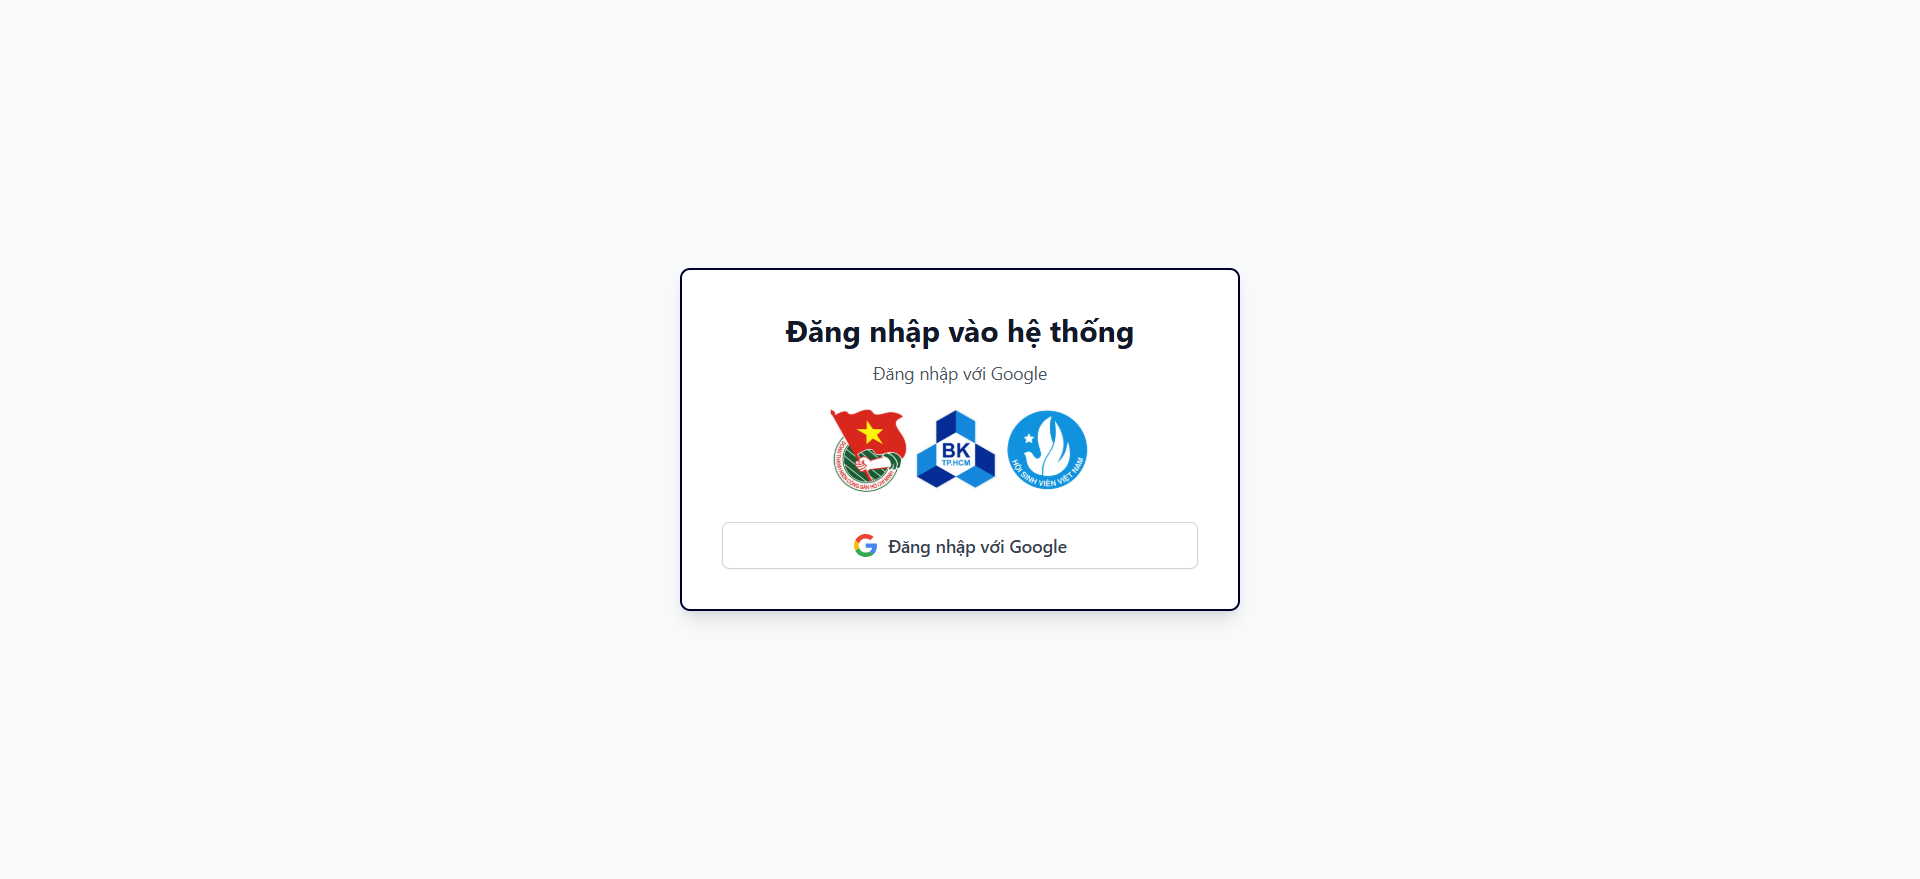
\includegraphics[width=0.96\linewidth]{Images/5.2 Hình giao diện/Đăng nhập/Login.png}
	\caption{Giao diện đăng nhập hệ thống}
\end{figure}

\begin{figure}[H]
	\centering
	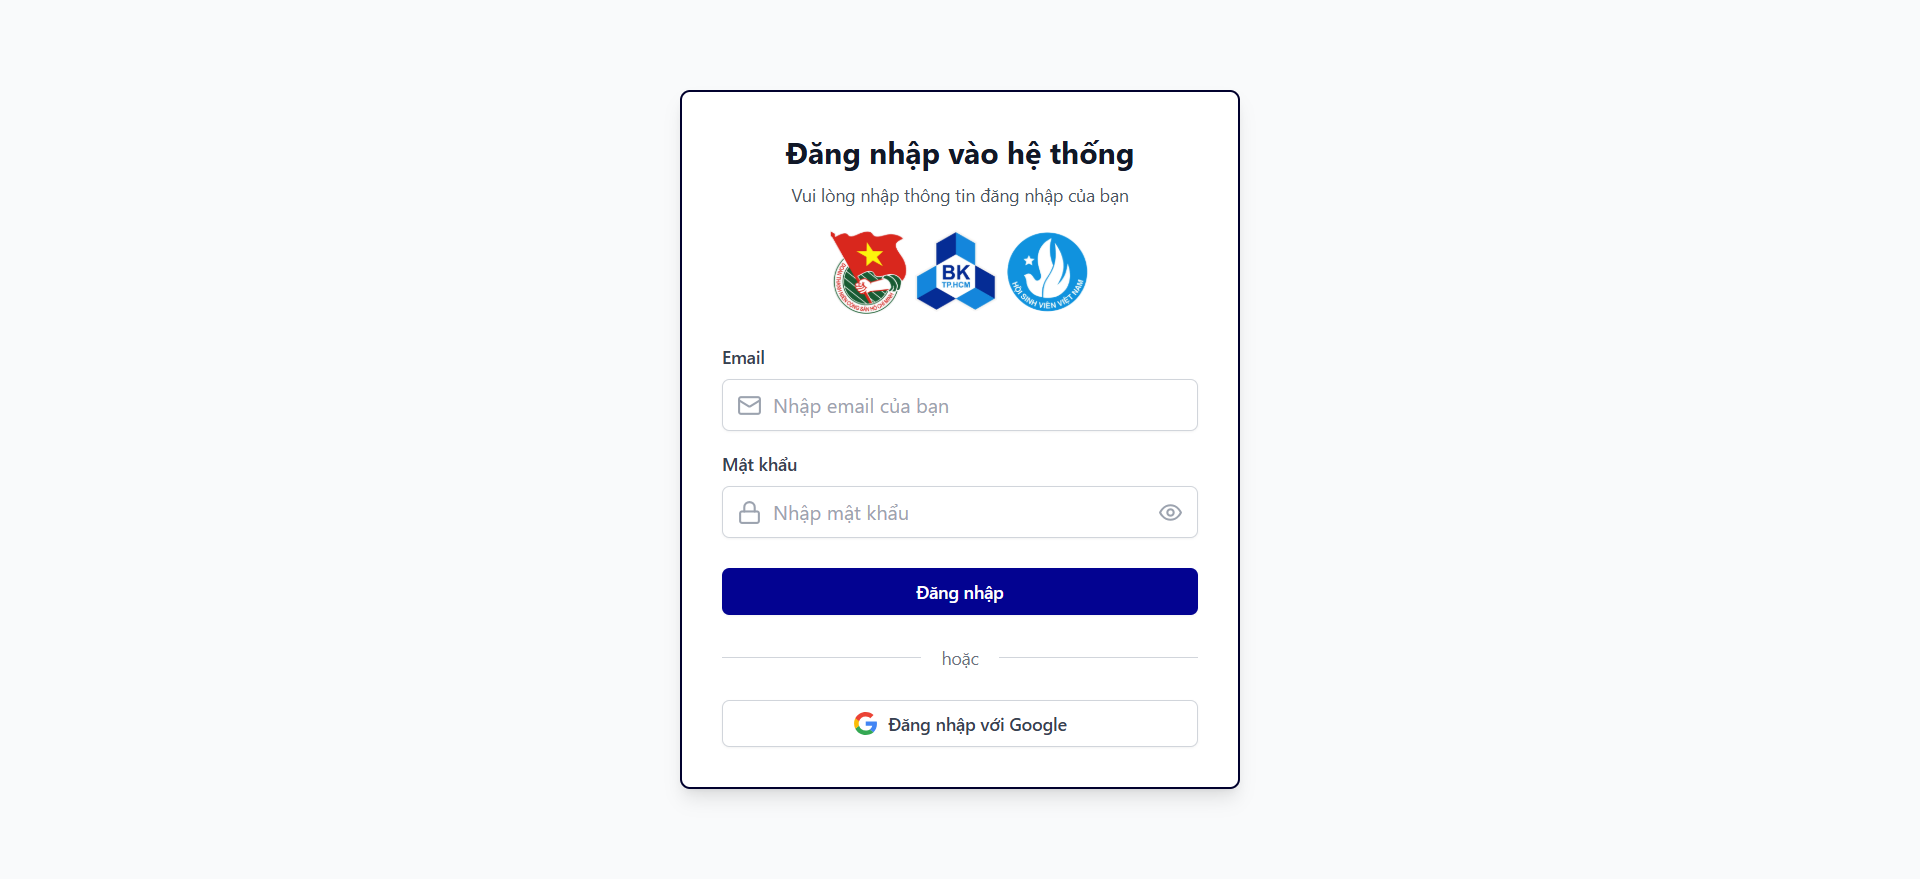
\includegraphics[width=0.96\linewidth]{Images/5.2 Hình giao diện/Đăng nhập/Login-Admin.png}
	\caption{Giao diện đăng nhập quản trị viên}
\end{figure}

\textbf{Nhóm dashboard và cấu hình hệ thống.}
\begin{figure}[H]
	\centering
	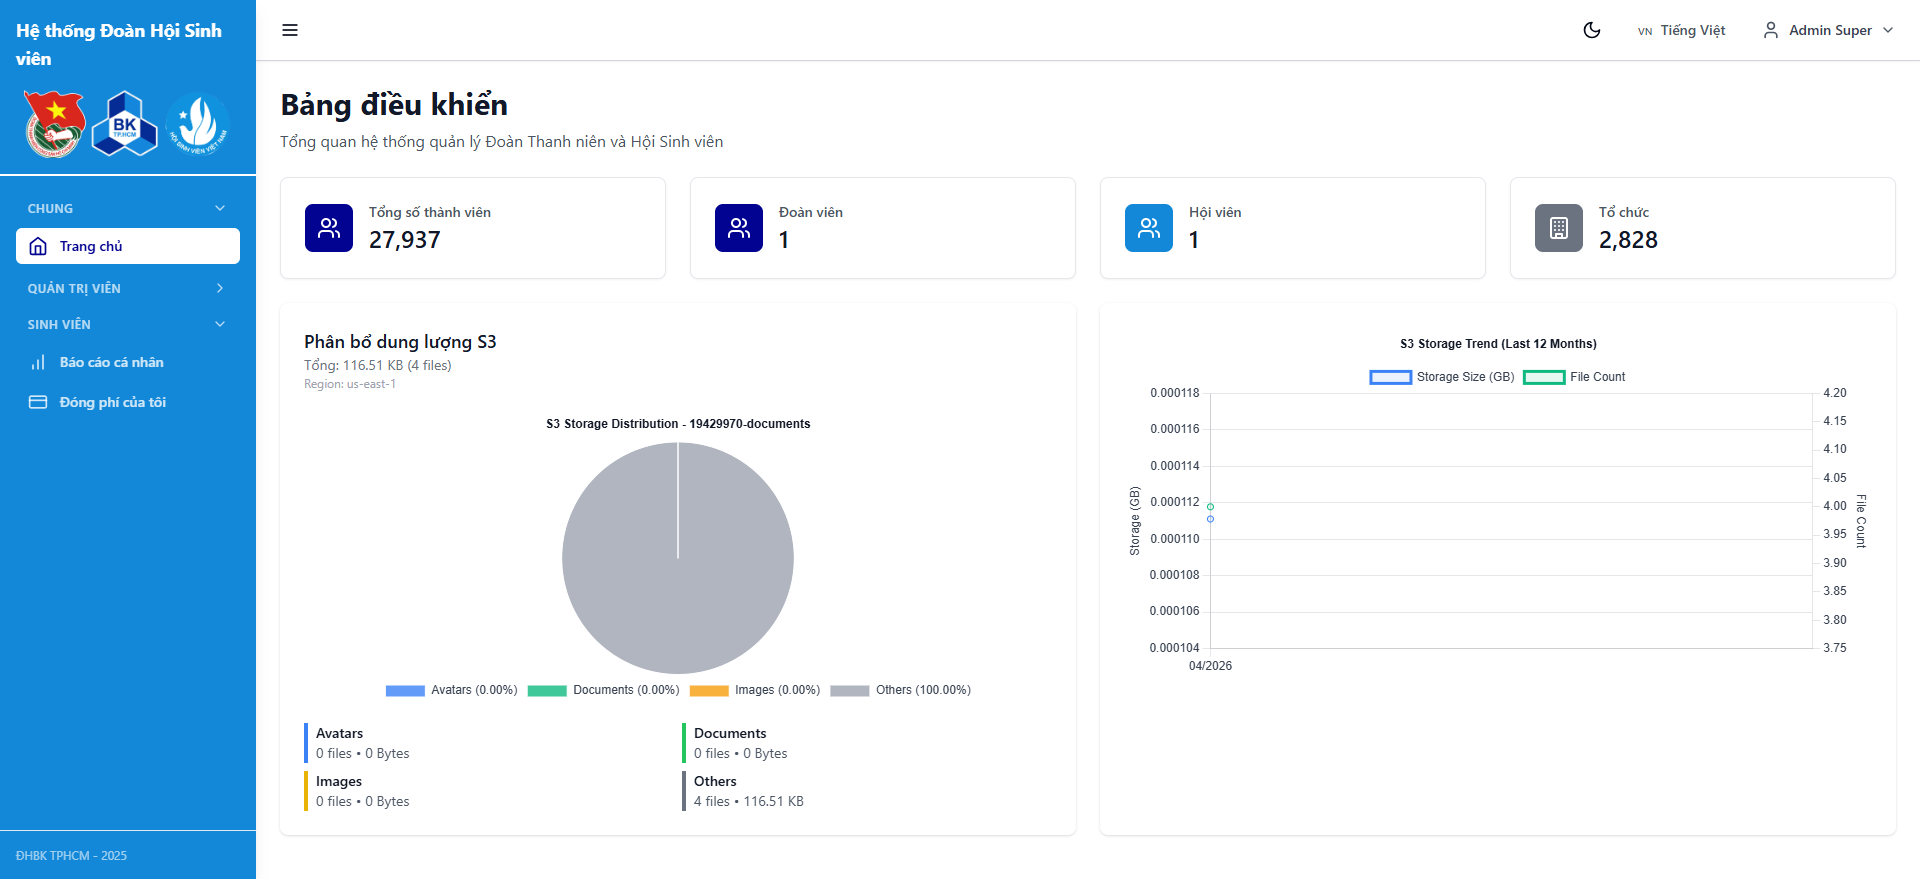
\includegraphics[width=0.96\linewidth]{Images/5.2 Hình giao diện/Dashboard.png}
	\caption{Giao diện dashboard tổng quan}
\end{figure}

\begin{figure}[H]
	\centering
	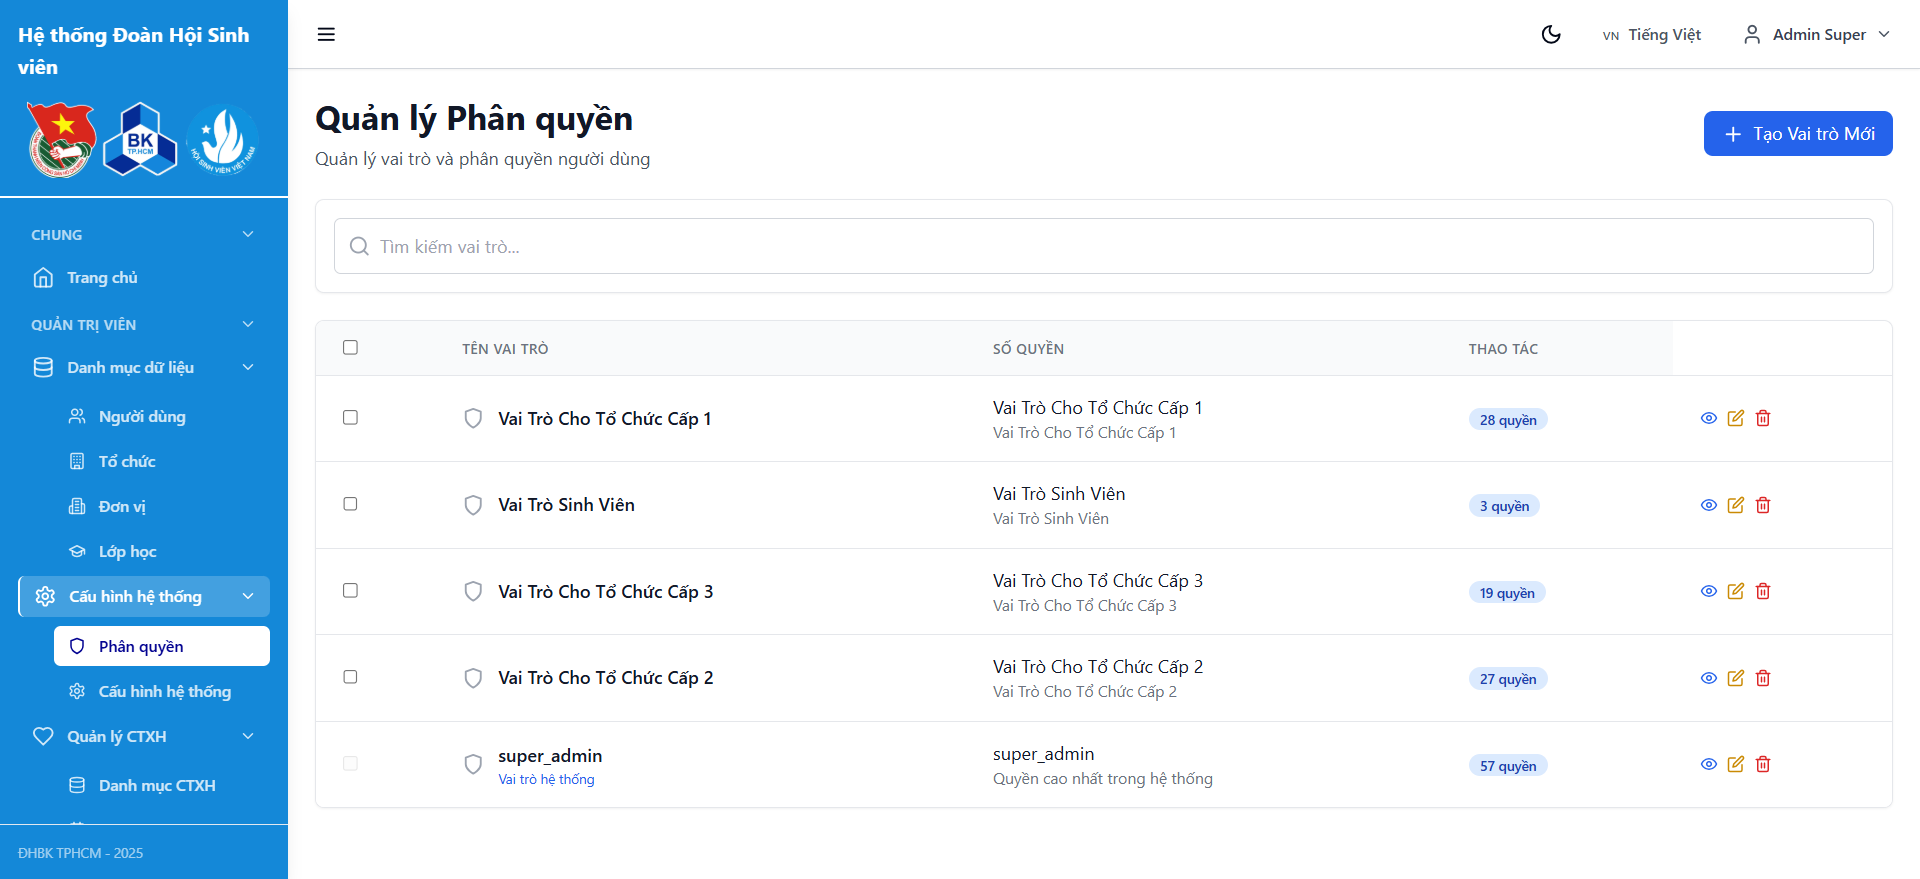
\includegraphics[width=0.96\linewidth]{Images/5.2 Hình giao diện/Phân quyền RBAC.png}
	\caption{Màn hình quản lý phân quyền RBAC}
\end{figure}

\begin{figure}[H]
	\centering
	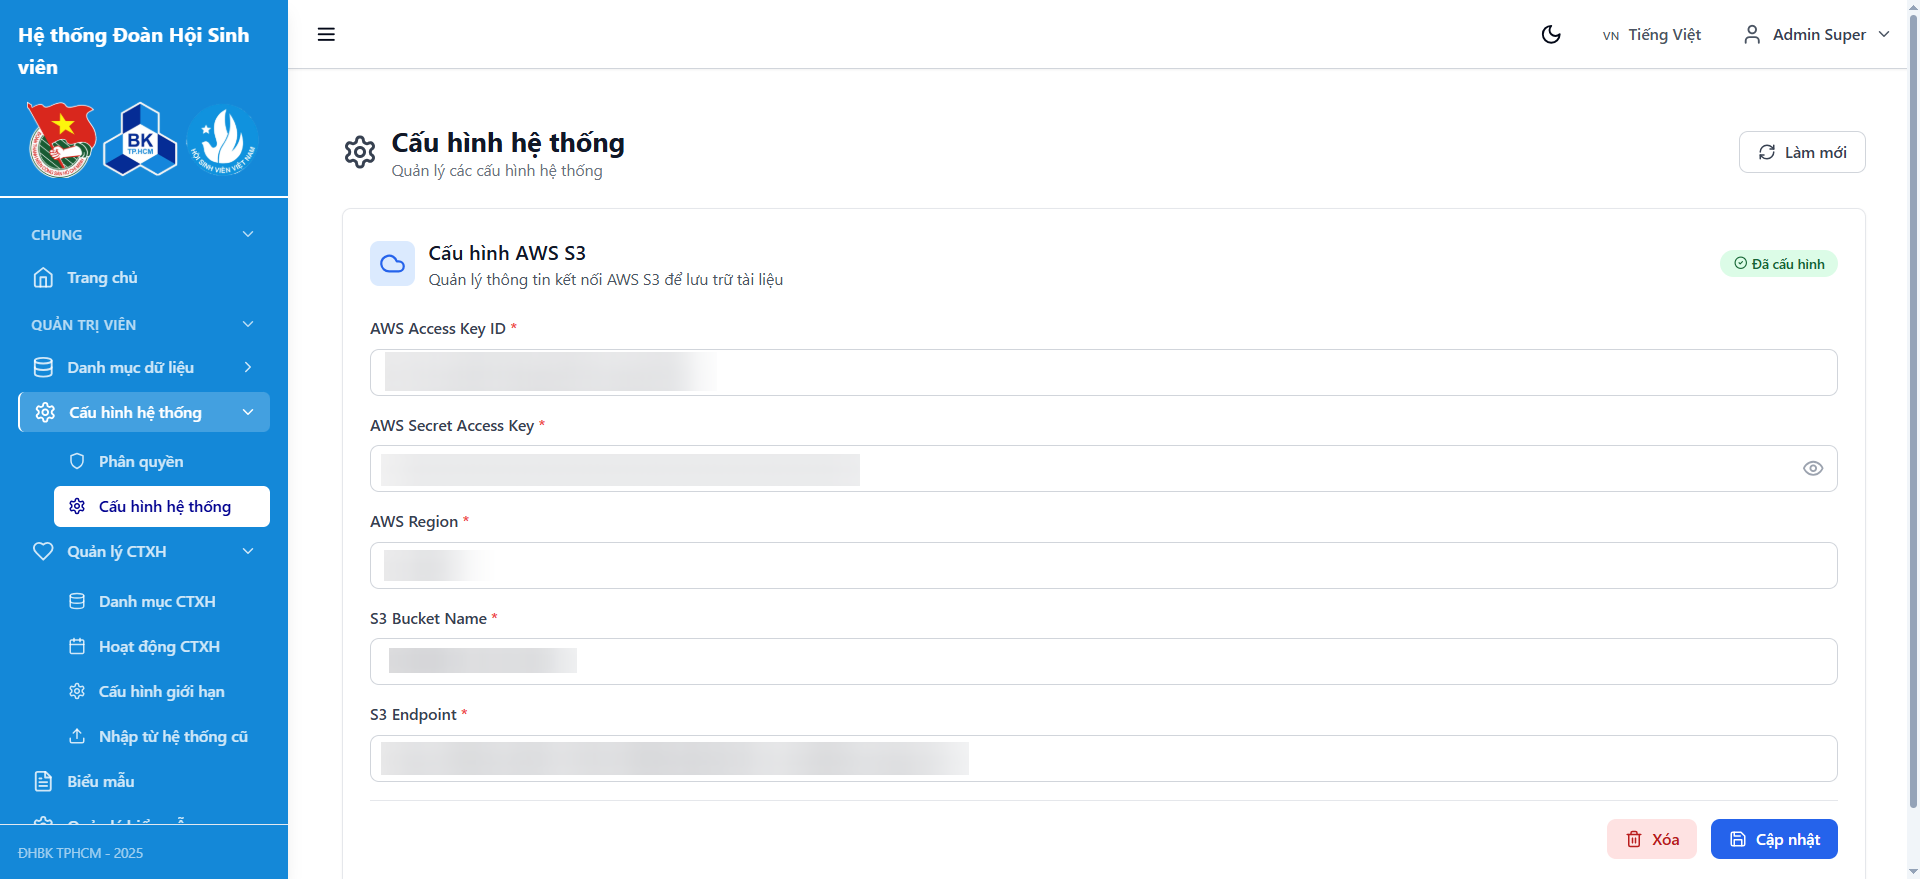
\includegraphics[width=0.96\linewidth]{Images/5.2 Hình giao diện/S3 config.png}
	\caption{Màn hình cấu hình hệ thống S3}
\end{figure}

\textbf{Nhóm quản trị dữ liệu nền.}
\begin{figure}[H]
	\centering
	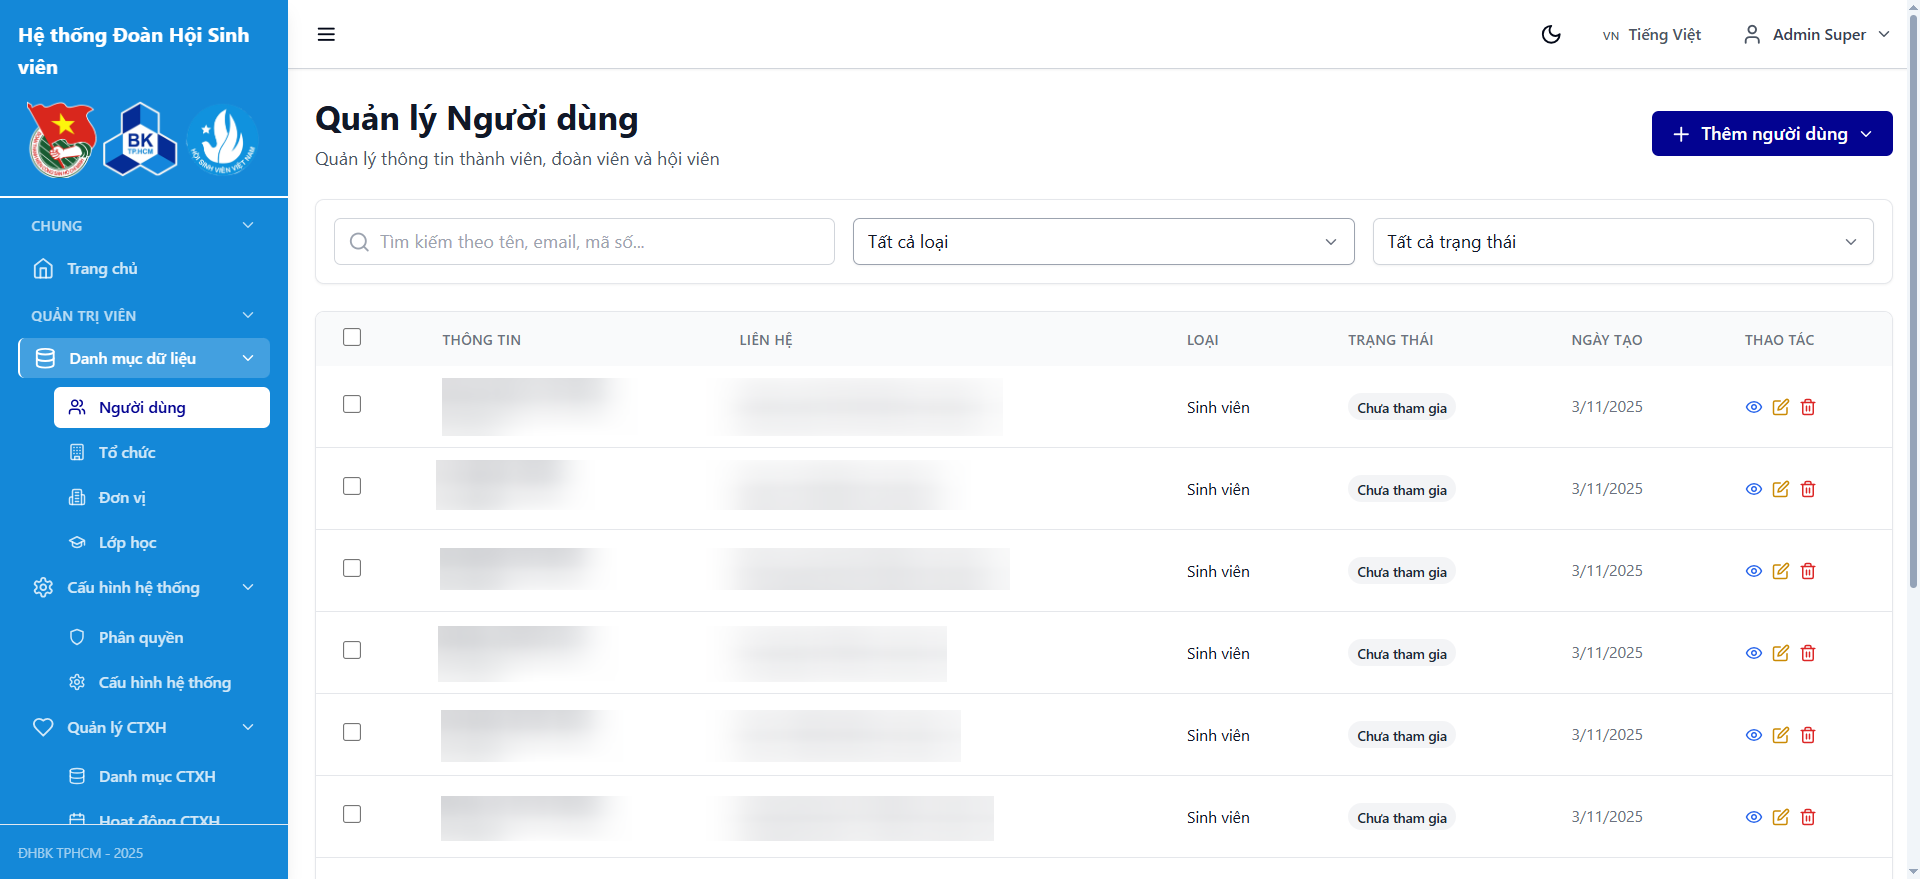
\includegraphics[width=0.96\linewidth]{Images/5.2 Hình giao diện/Danh mục dữ liệu/Users.png}
	\caption{Giao diện quản lý người dùng}
\end{figure}

\begin{figure}[H]
	\centering
	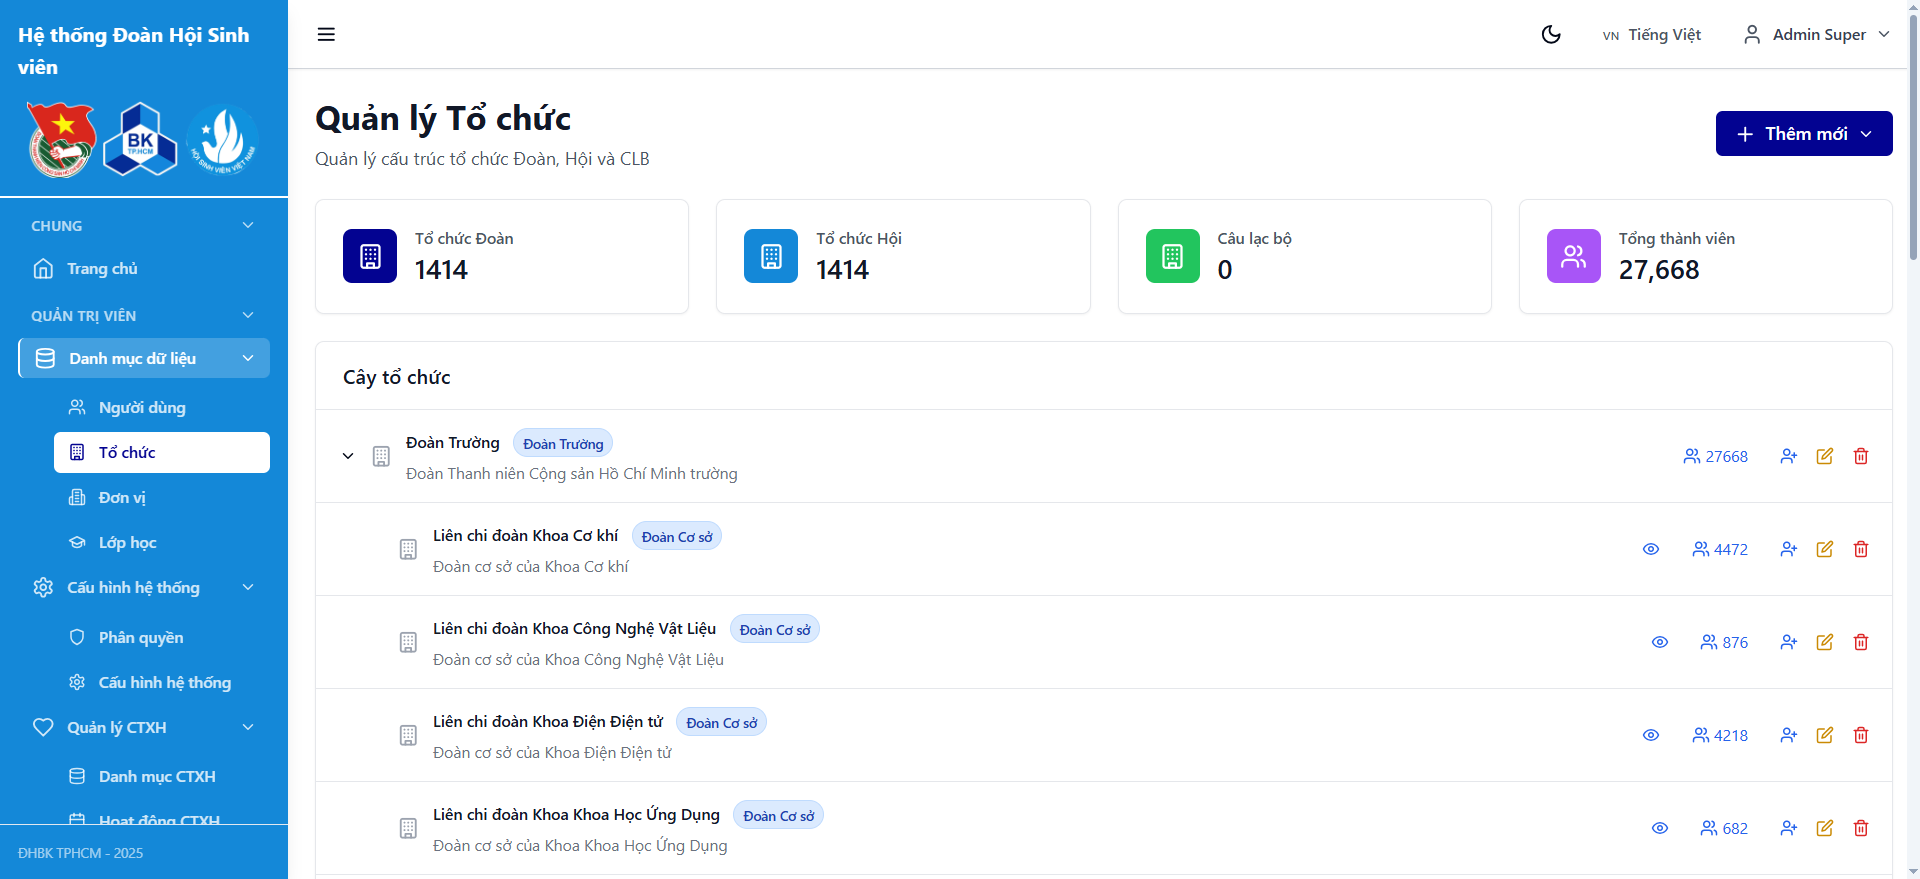
\includegraphics[width=0.96\linewidth]{Images/5.2 Hình giao diện/Danh mục dữ liệu/Organizations.png}
	\caption{Giao diện quản lý tổ chức}
\end{figure}

\begin{figure}[H]
	\centering
	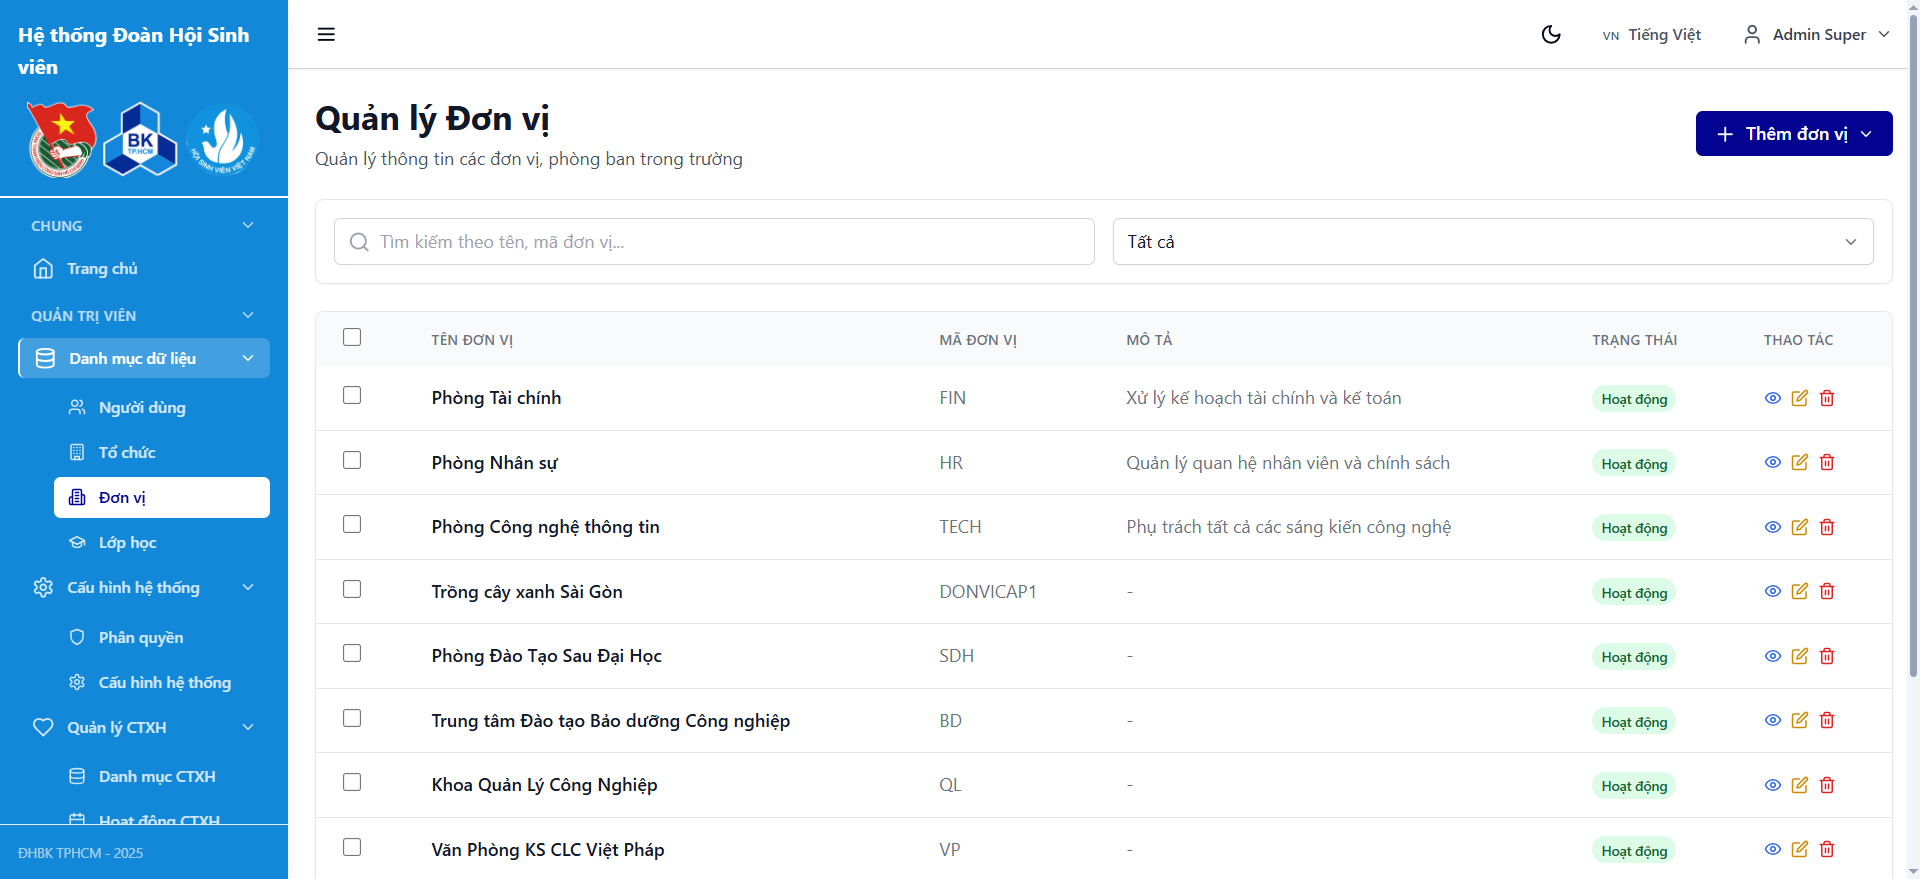
\includegraphics[width=0.96\linewidth]{Images/5.2 Hình giao diện/Danh mục dữ liệu/Departments.png}
	\caption{Giao diện quản lý đơn vị/khoa}
\end{figure}

\begin{figure}[H]
	\centering
	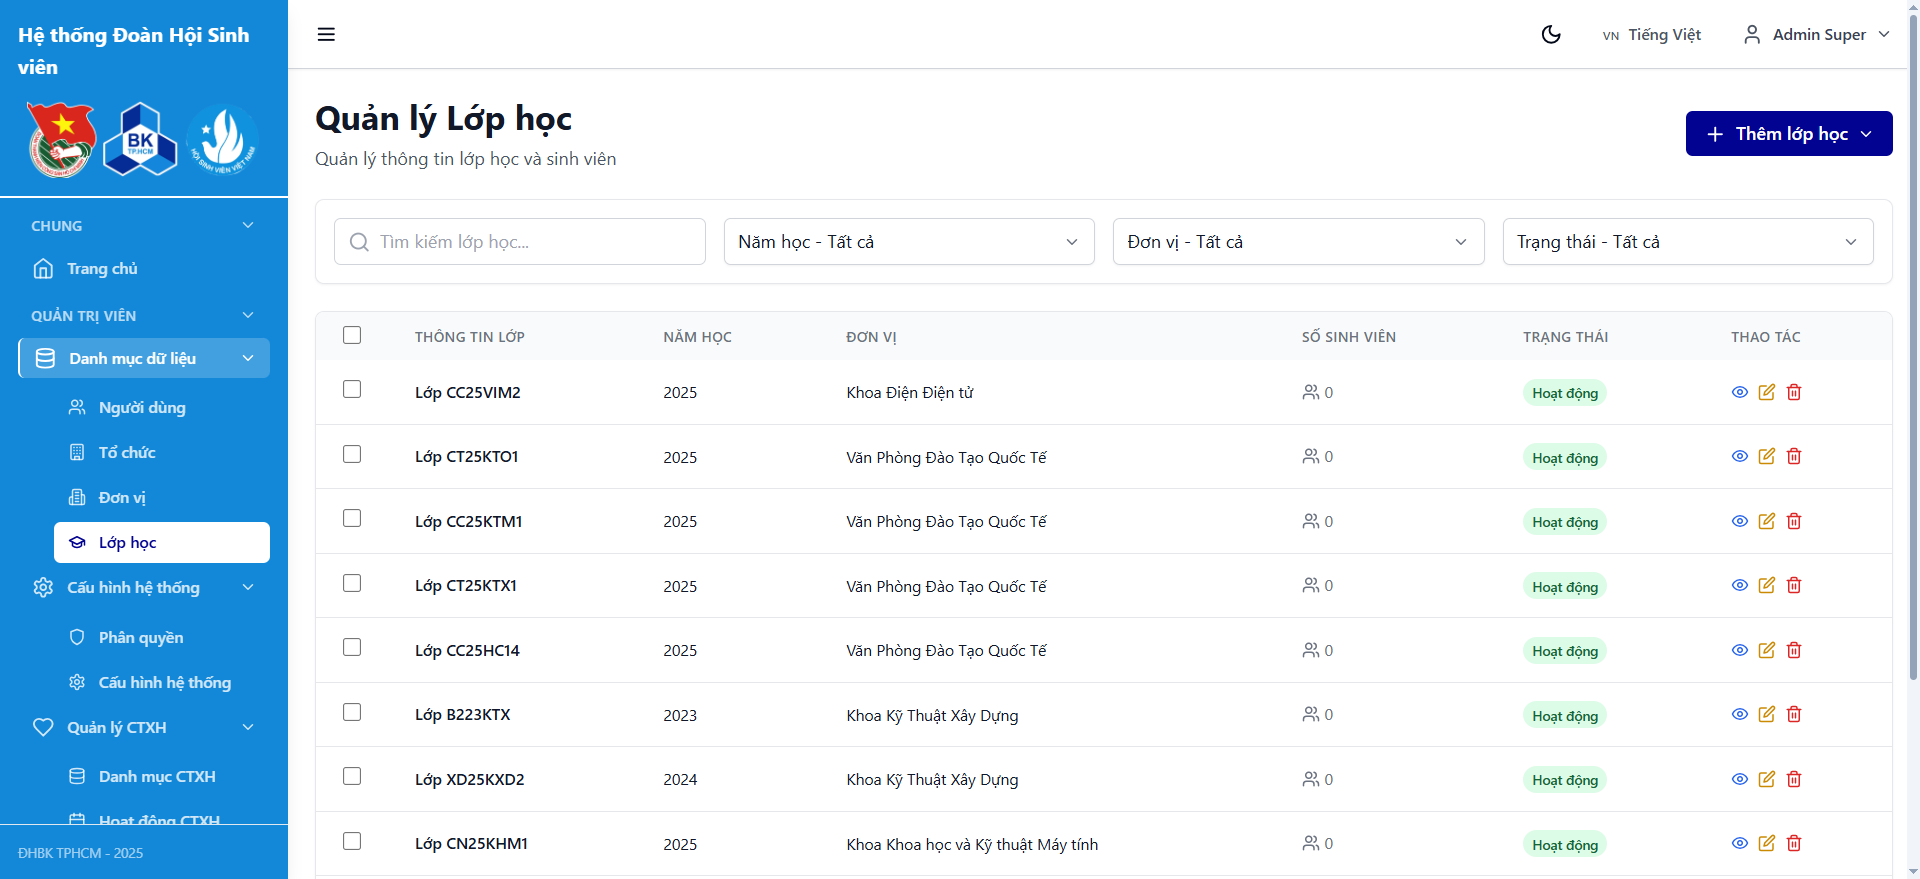
\includegraphics[width=0.96\linewidth]{Images/5.2 Hình giao diện/Danh mục dữ liệu/Classes.png}
	\caption{Giao diện quản lý lớp học}
\end{figure}

\textbf{Nhóm quản lý công tác xã hội.}
\begin{figure}[H]
	\centering
	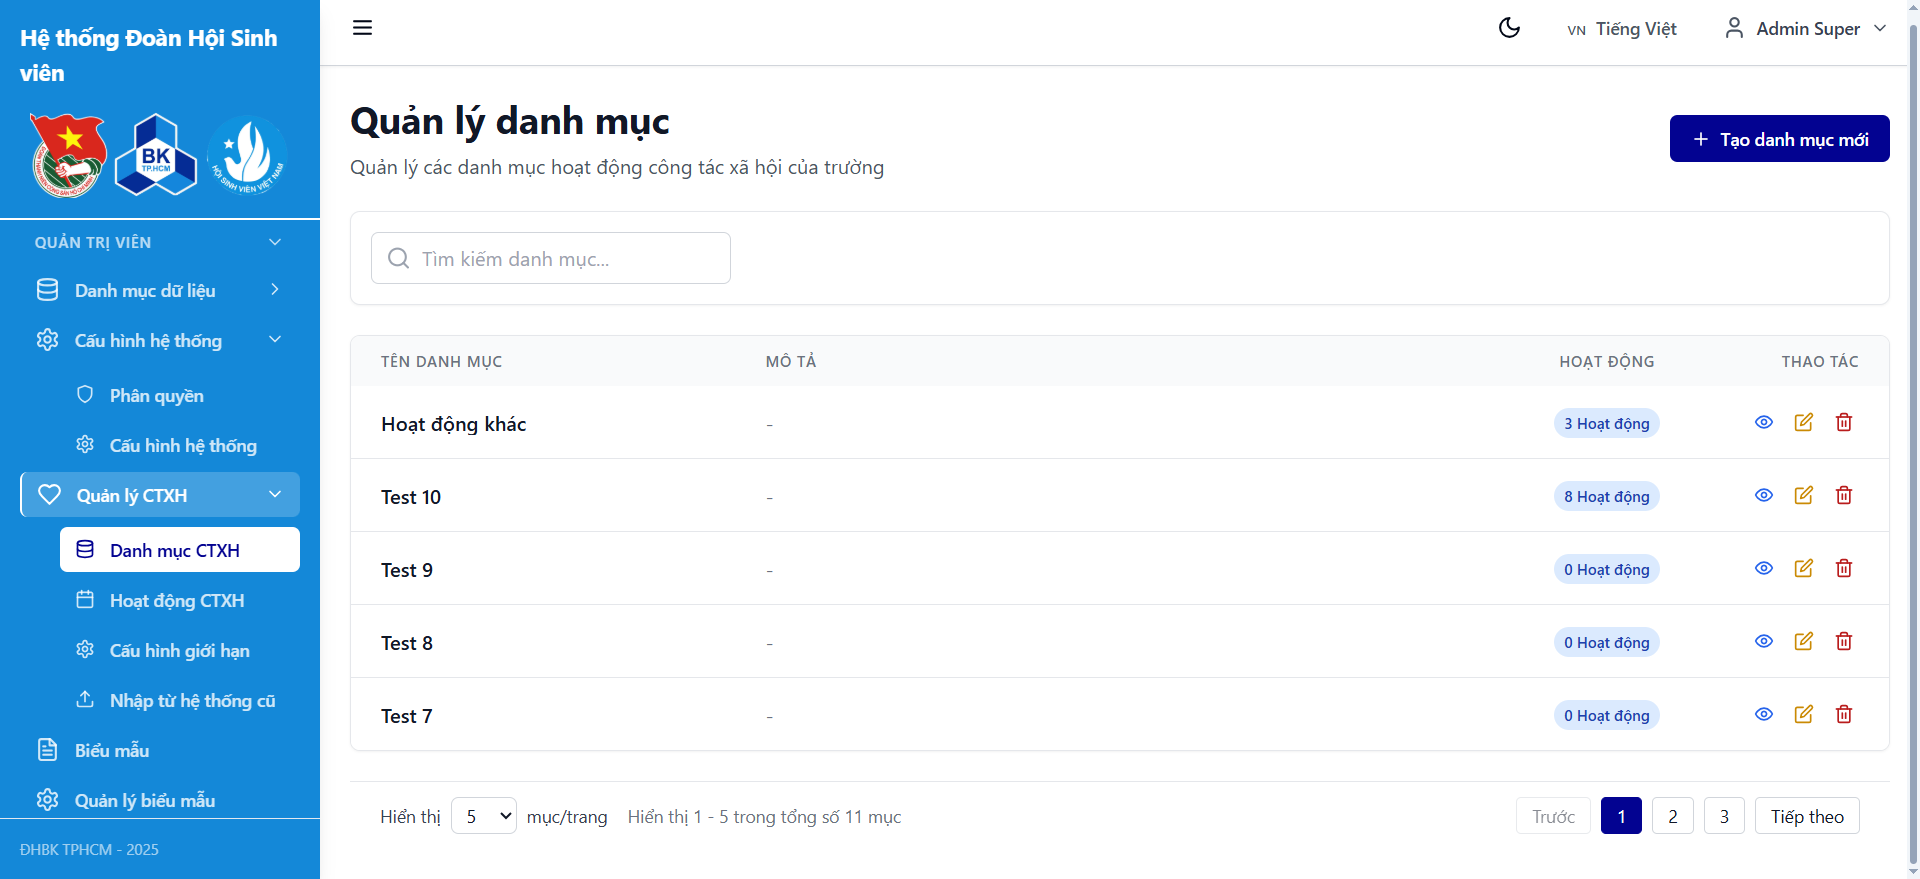
\includegraphics[width=0.96\linewidth]{Images/5.2 Hình giao diện/CTXH/CTXH-Categories.png}
	\caption{Giao diện quản lý danh mục CTXH}
\end{figure}

\begin{figure}[H]
	\centering
	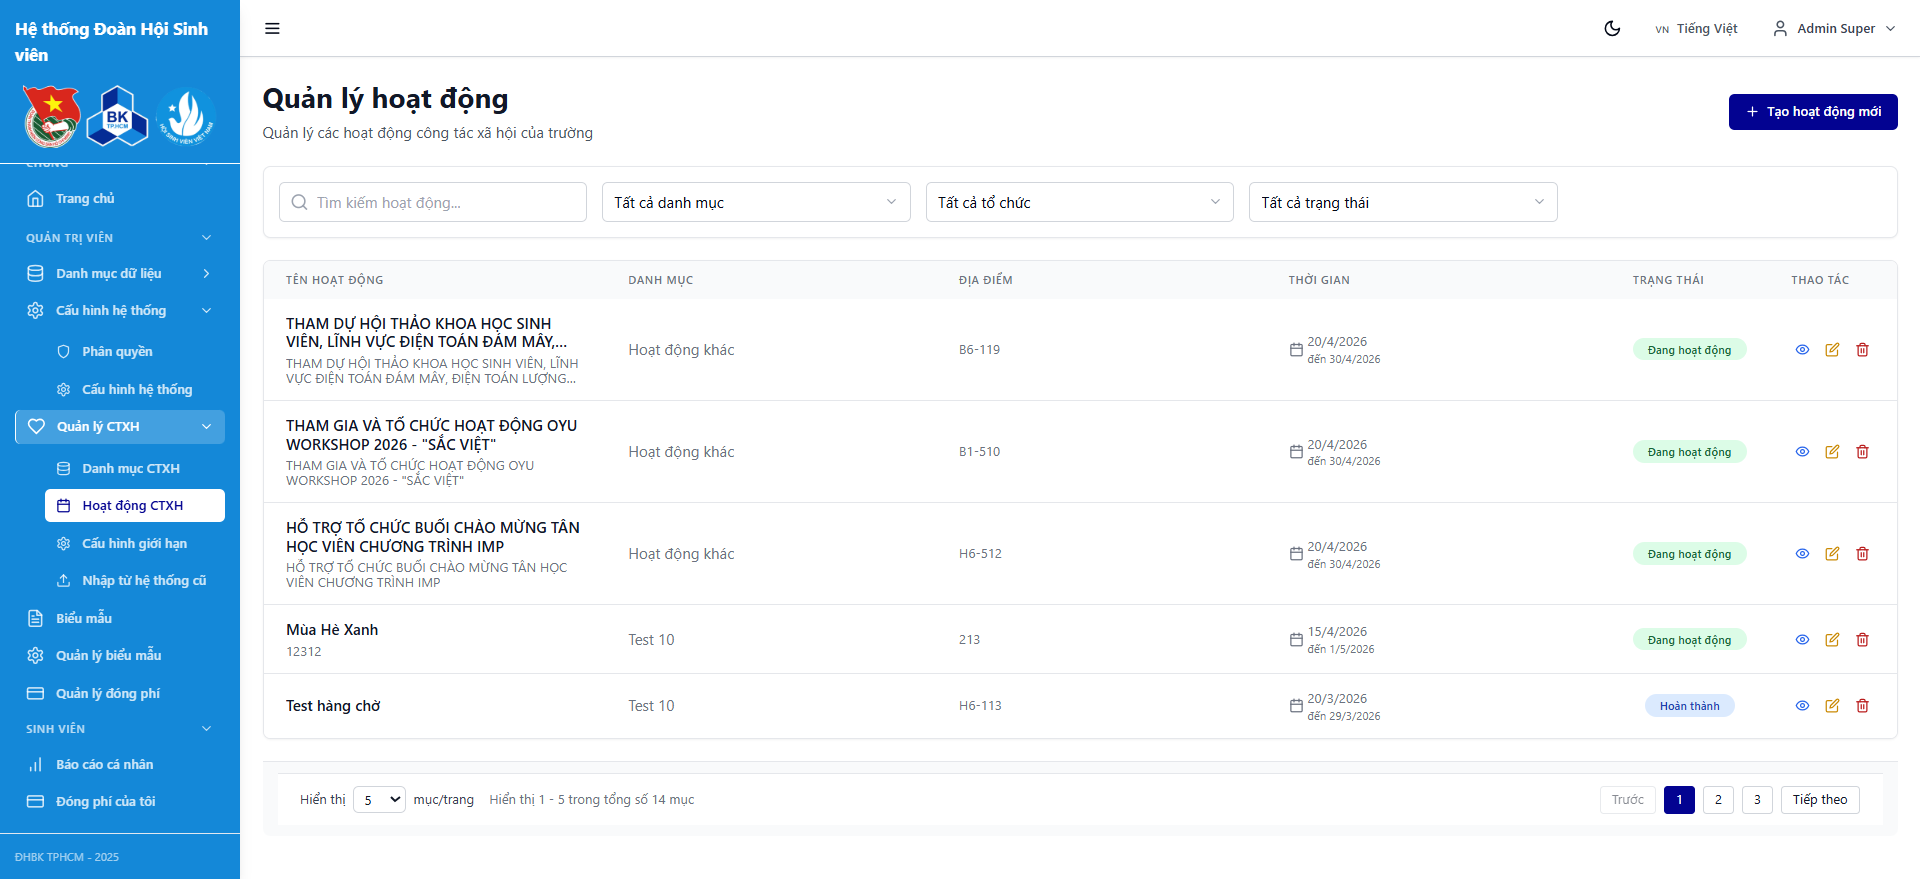
\includegraphics[width=0.96\linewidth]{Images/5.2 Hình giao diện/CTXH/CTXH-Activities.png}
	\caption{Giao diện quản lý hoạt động CTXH theo danh mục}
\end{figure}

\begin{figure}[H]
	\centering
	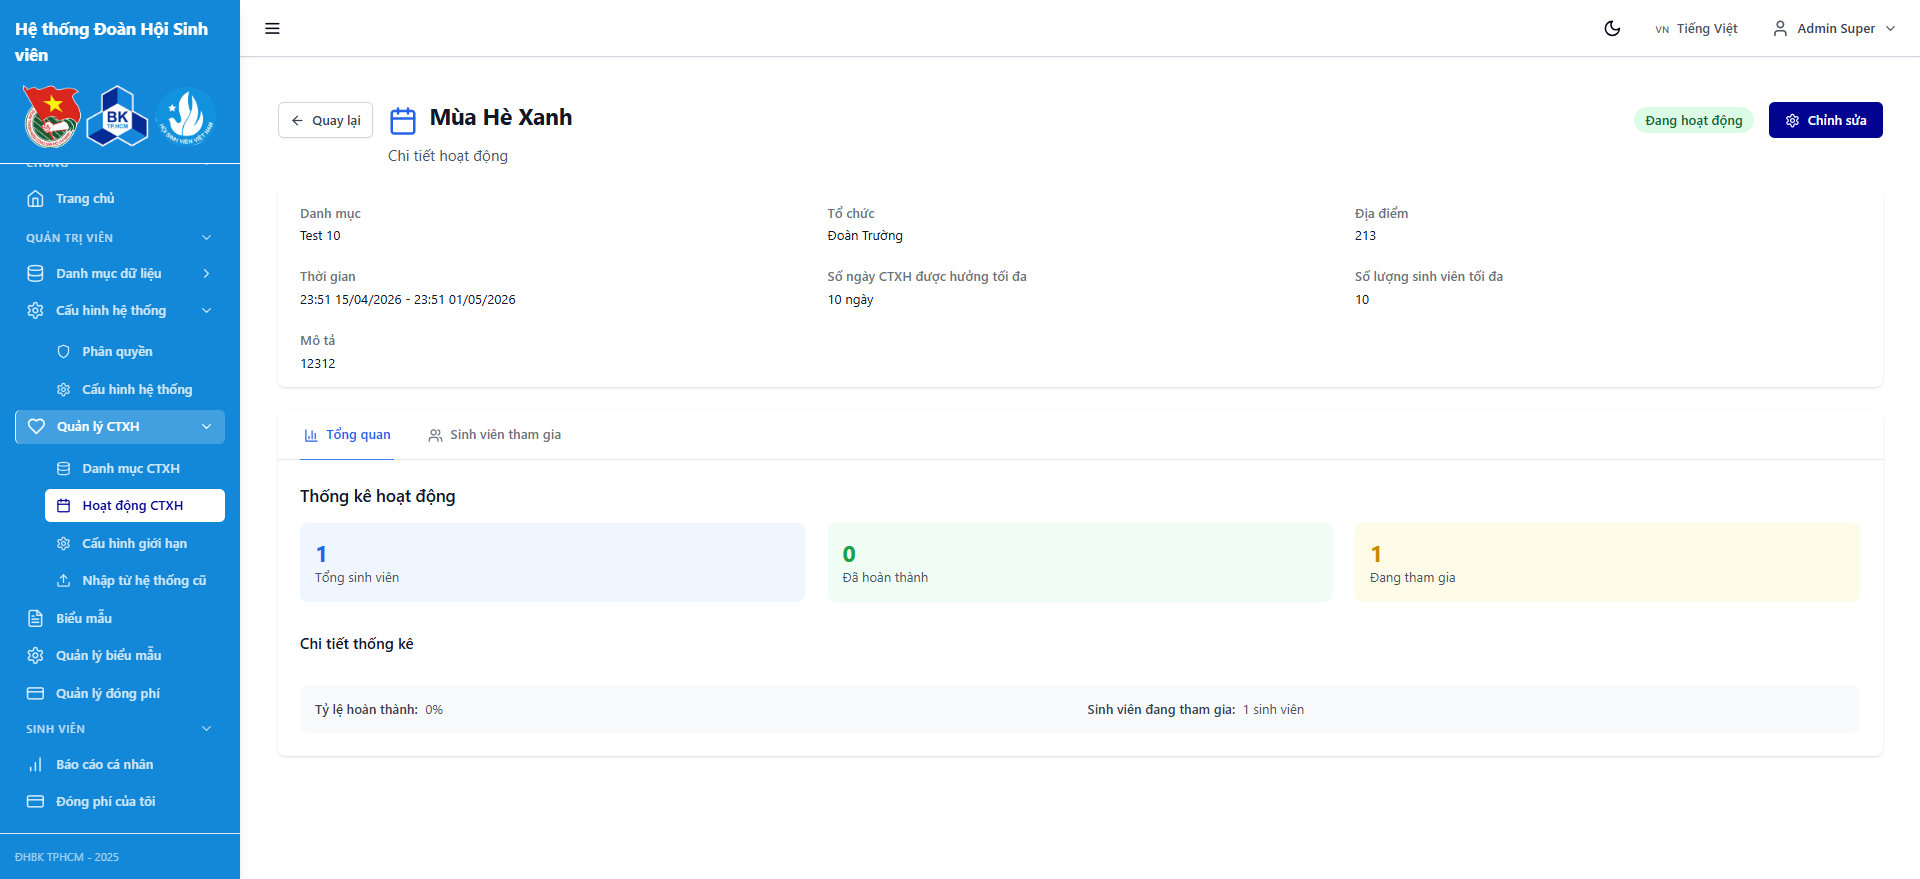
\includegraphics[width=0.96\linewidth]{Images/5.2 Hình giao diện/CTXH/Participant - Tổng quan.png}
	\caption{Giao diện chi tiết hoạt động (tab tổng quan)}
\end{figure}

\begin{figure}[H]
	\centering
	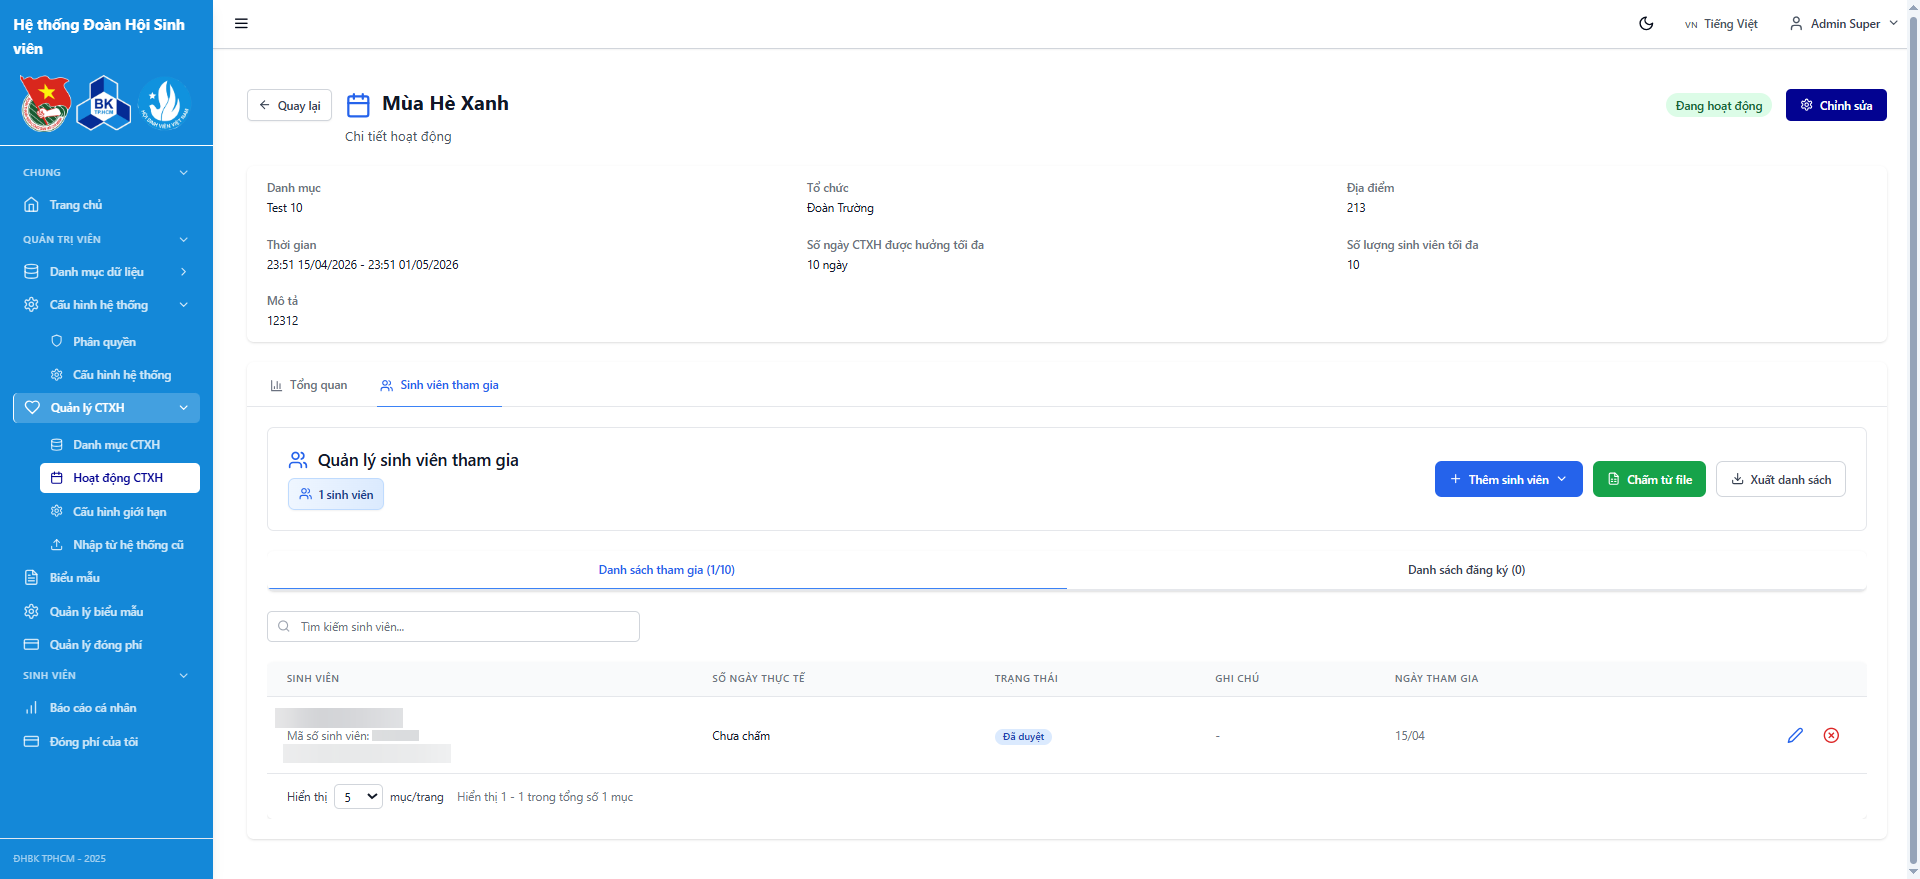
\includegraphics[width=0.96\linewidth]{Images/5.2 Hình giao diện/CTXH/Participant - Danh sách tham gia.png}
	\caption{Giao diện danh sách sinh viên tham gia hoạt động CTXH}
\end{figure}

\begin{figure}[H]
	\centering
	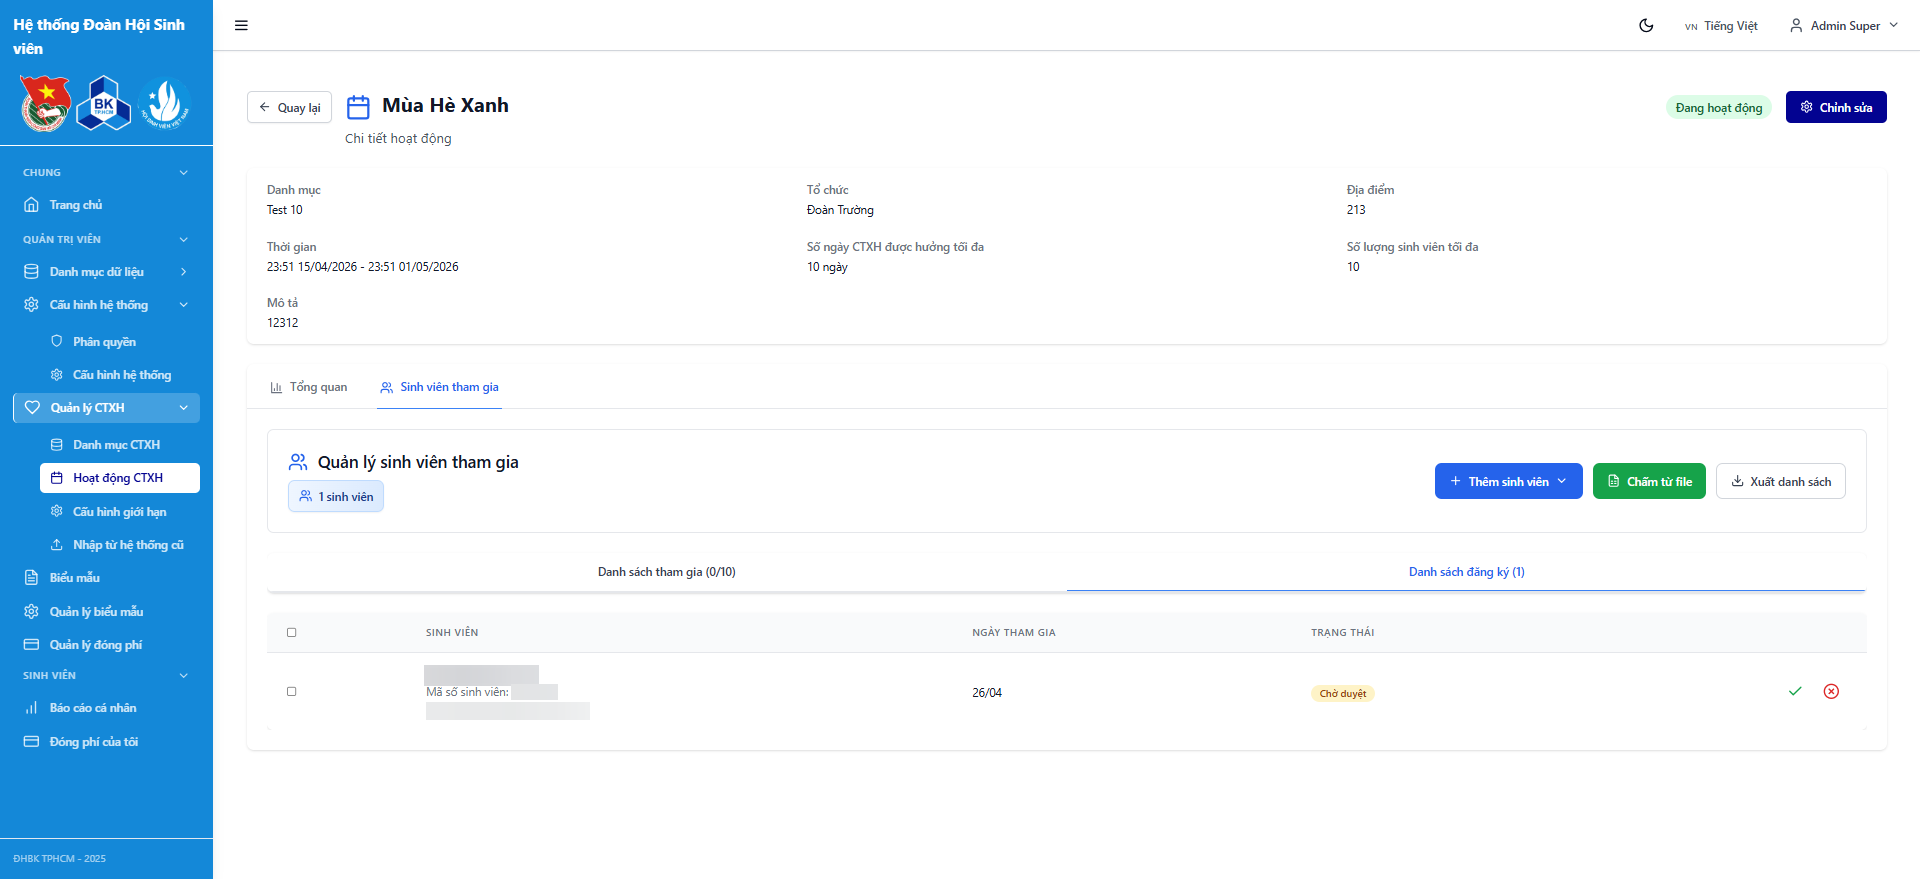
\includegraphics[width=0.96\linewidth]{Images/5.2 Hình giao diện/CTXH/Participant - Danh sách đăng ký chờ duyệt.png}
	\caption{Giao diện danh sách đăng ký chờ duyệt của hoạt động CTXH}
\end{figure}

\begin{figure}[H]
	\centering
	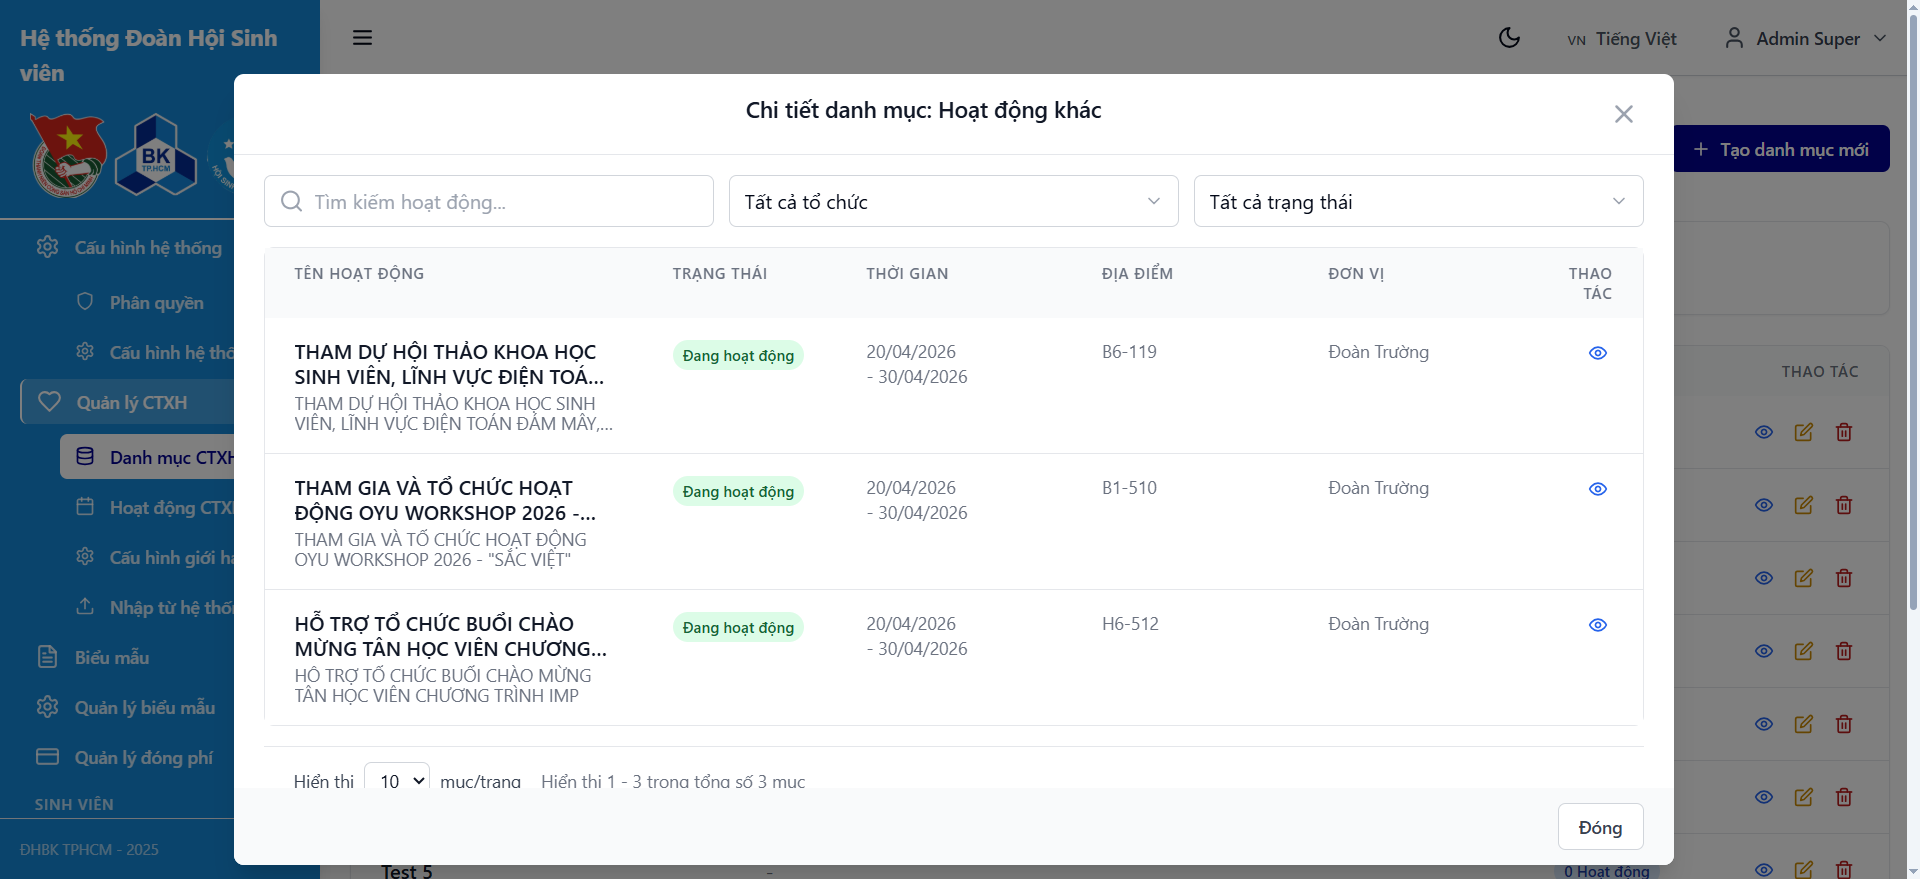
\includegraphics[width=0.96\linewidth]{Images/5.2 Hình giao diện/CTXH/CTXH-Category detail.png}
	\caption{Màn hình xem chi tiết danh mục và danh sách hoạt động thuộc danh mục}
\end{figure}

\begin{figure}[H]
	\centering
	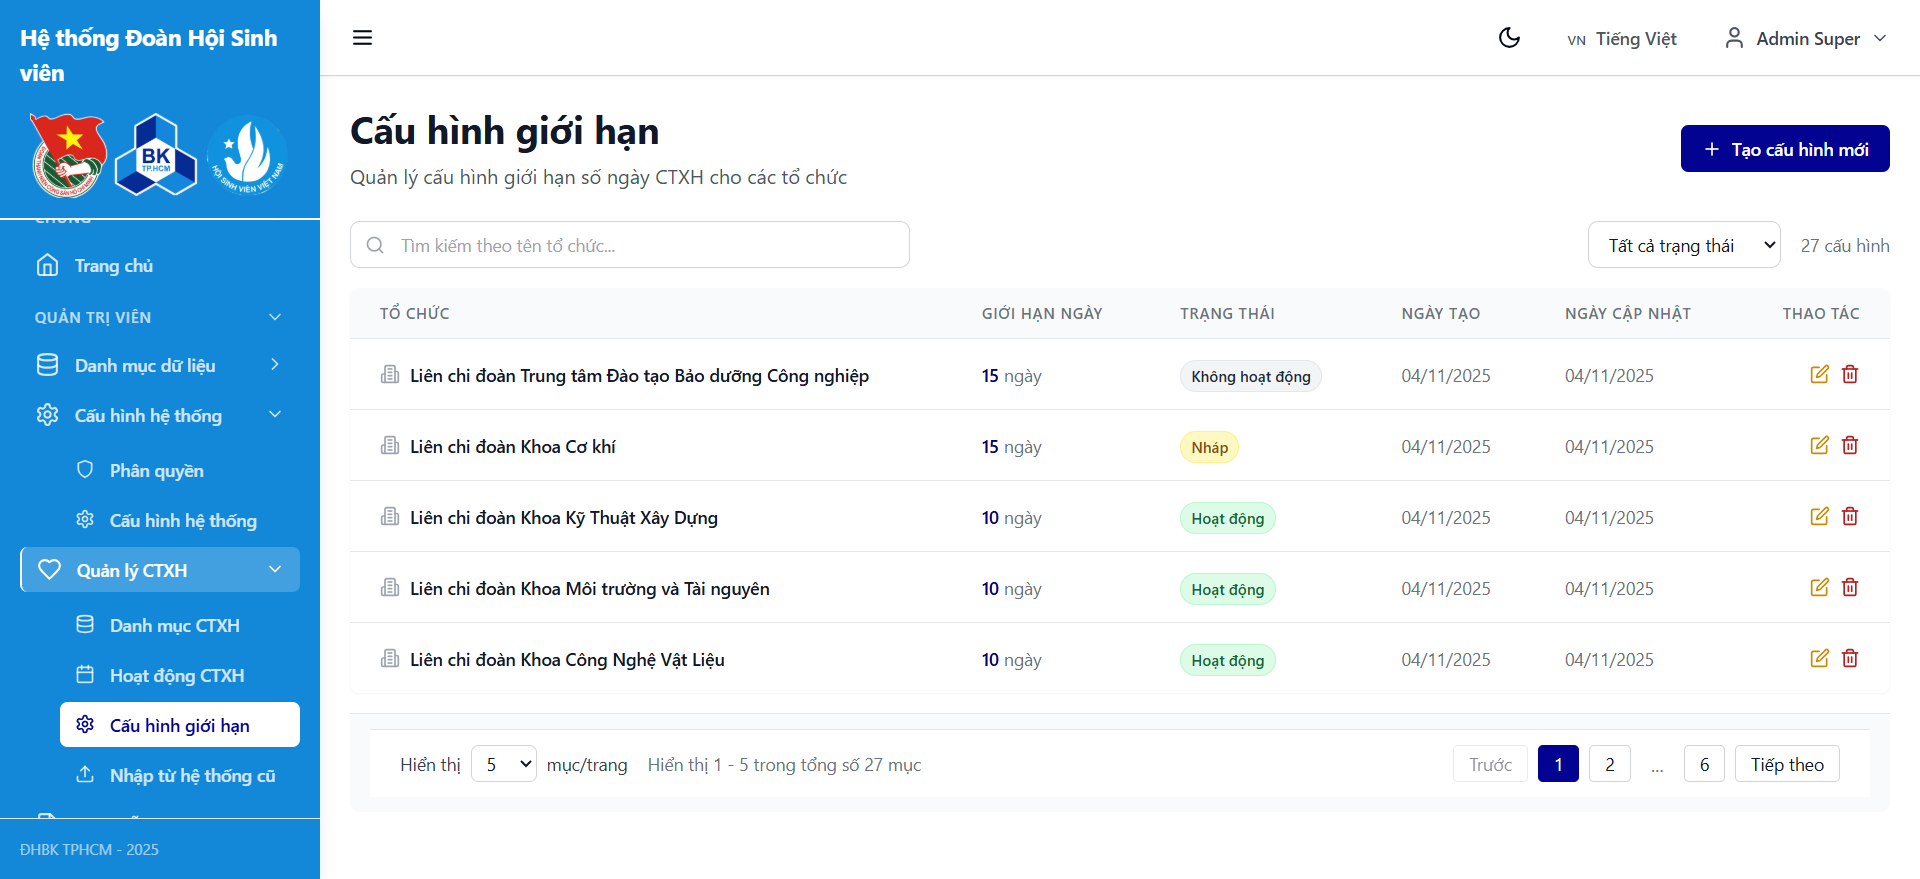
\includegraphics[width=0.96\linewidth]{Images/5.2 Hình giao diện/CTXH/CTXH-Limit Config.png}
	\caption{Giao diện cấu hình giới hạn ngày CTXH}
\end{figure}

\begin{figure}[H]
	\centering
	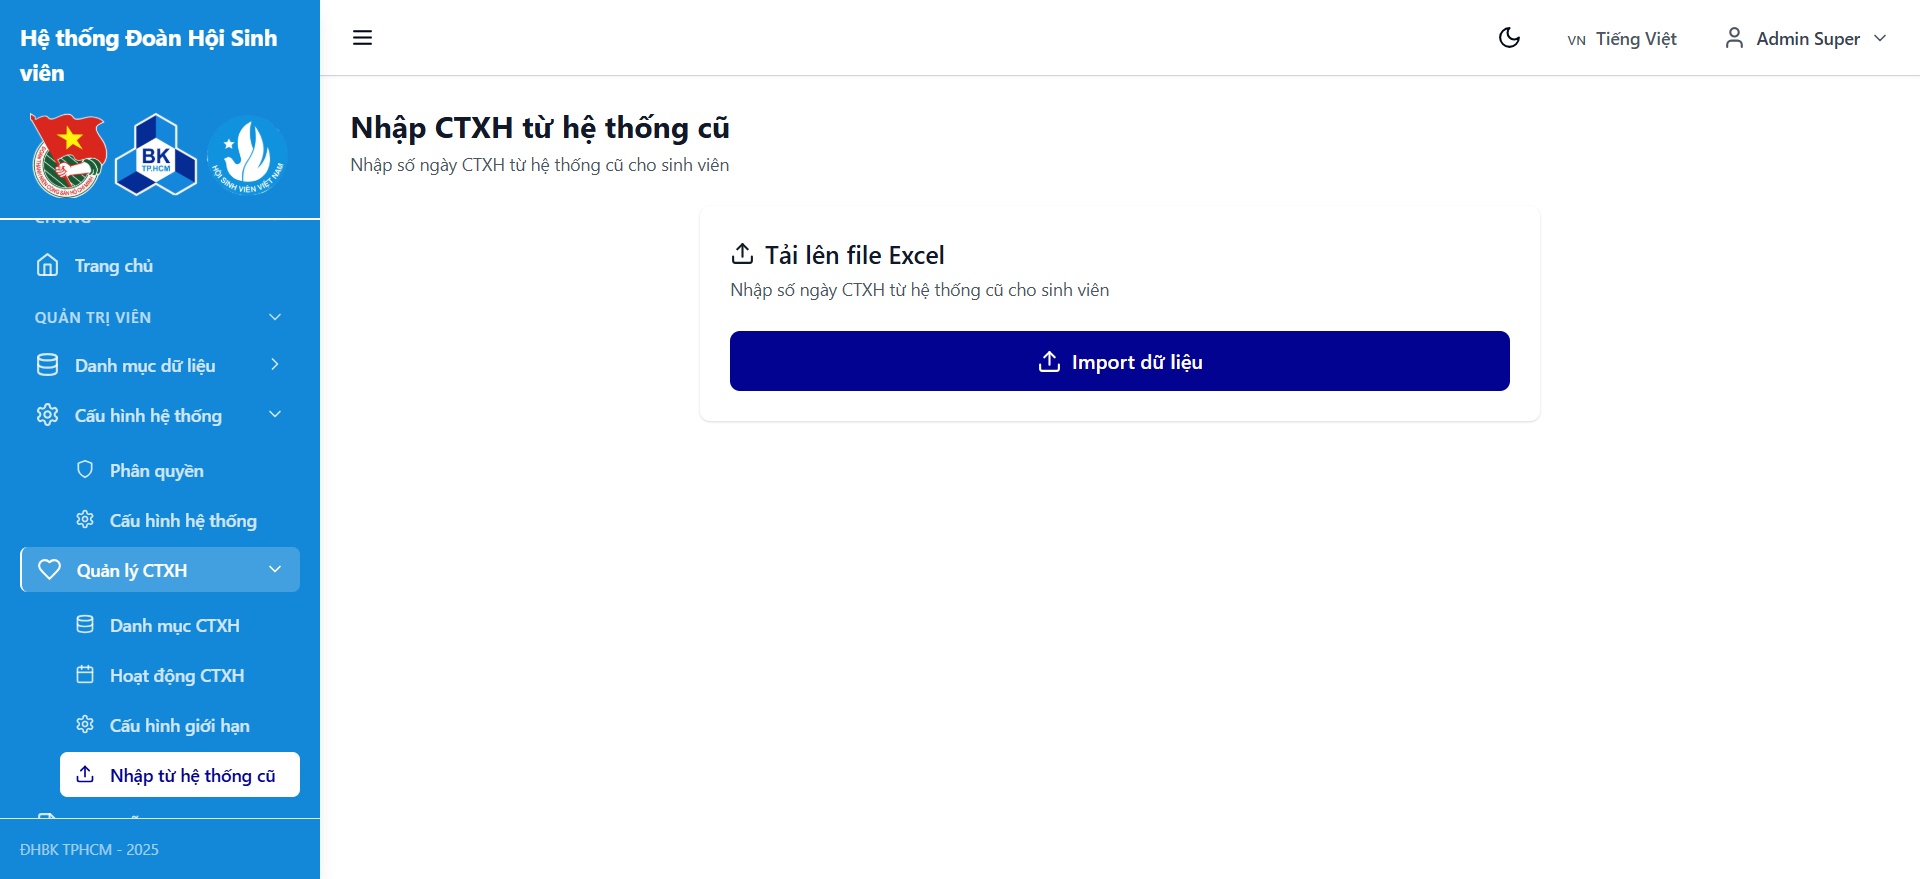
\includegraphics[width=0.96\linewidth]{Images/5.2 Hình giao diện/CTXH/CTXH- Import from old system.png}
	\caption{Giao diện nhập dữ liệu CTXH từ hệ thống cũ}
\end{figure}

\begin{figure}[H]
	\centering
	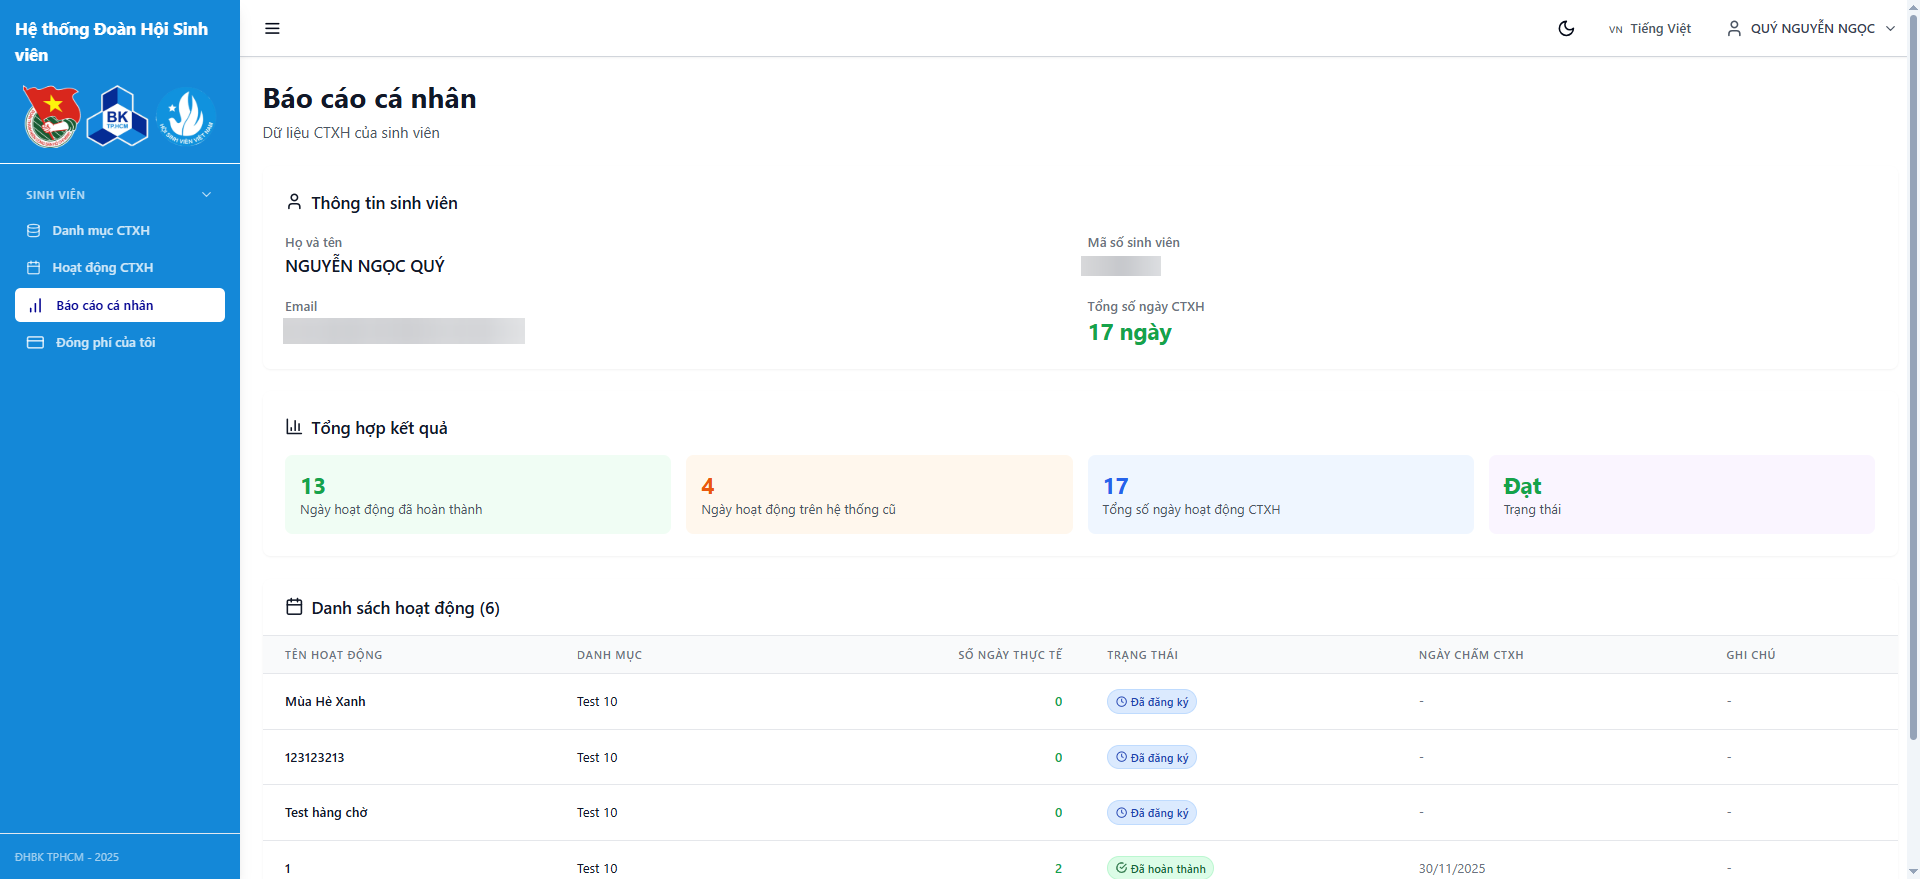
\includegraphics[width=0.96\linewidth]{Images/5.2 Hình giao diện/CTXH/CTXH - Student report.png}
	\caption{Giao diện báo cáo CTXH cá nhân của sinh viên}
\end{figure}

\textbf{Nhóm thu phí.}
\begin{figure}[H]
	\centering
	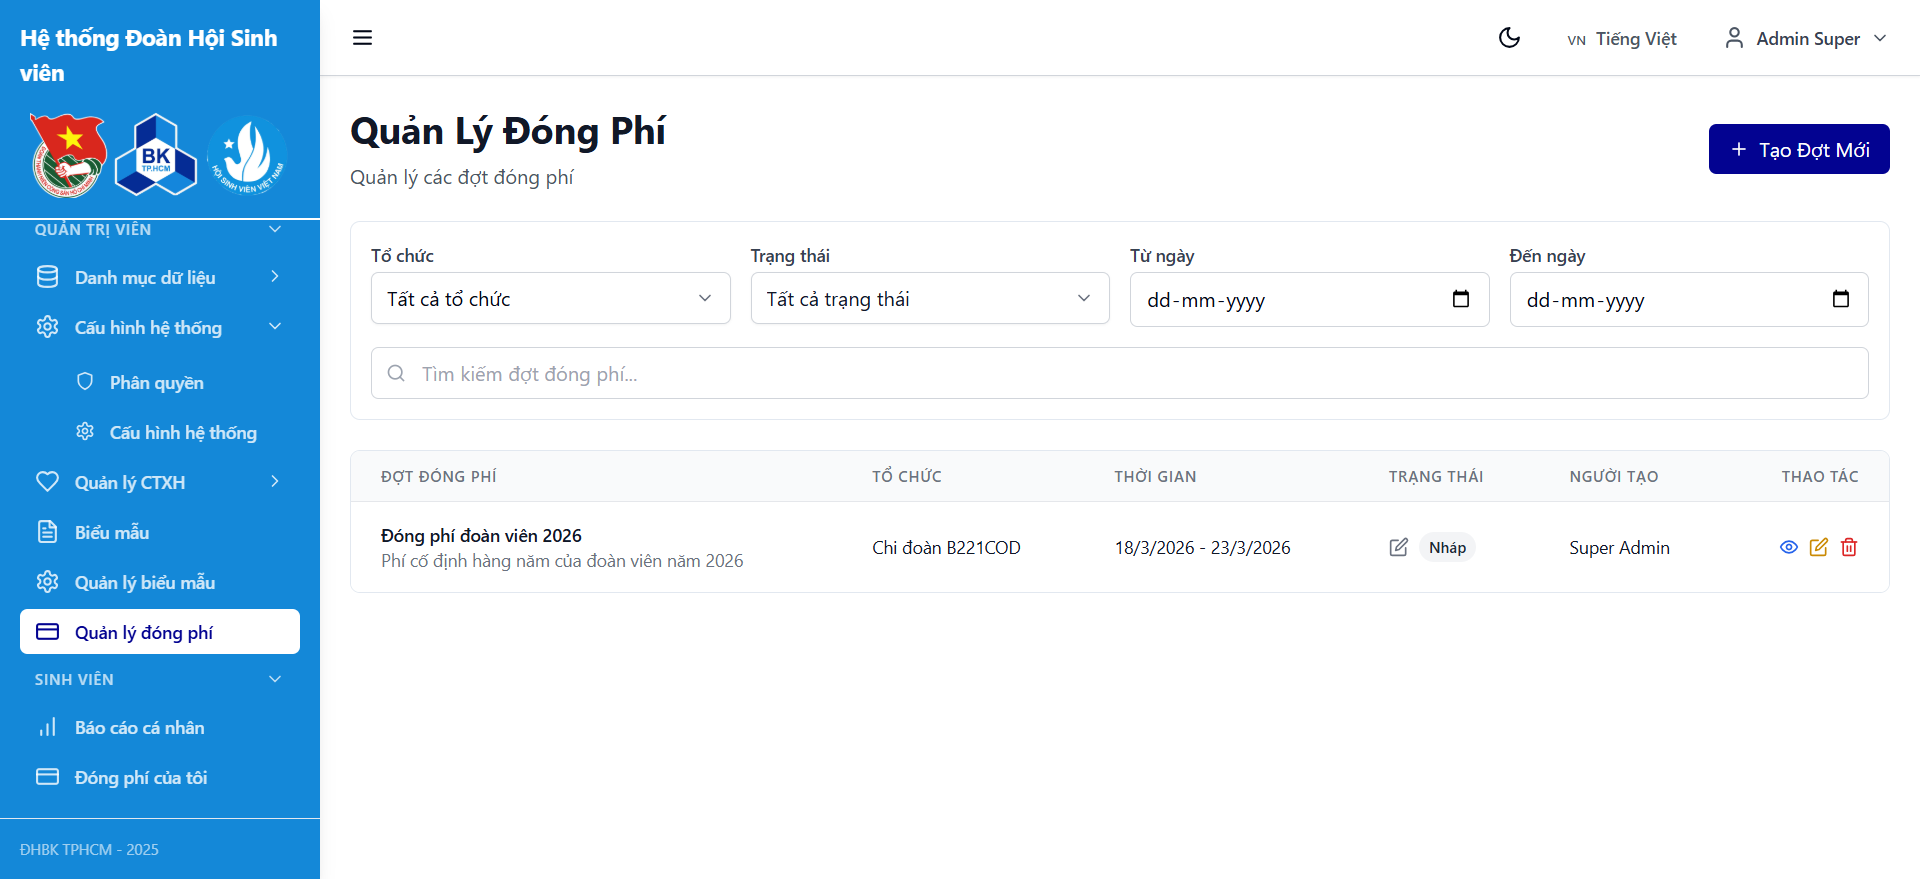
\includegraphics[width=0.96\linewidth]{Images/5.2 Hình giao diện/Module Thu phí/Trang Quản lý đóng phí.png}
	\caption{Giao diện quản lý đóng phí theo đợt}
\end{figure}

\begin{figure}[H]
	\centering
	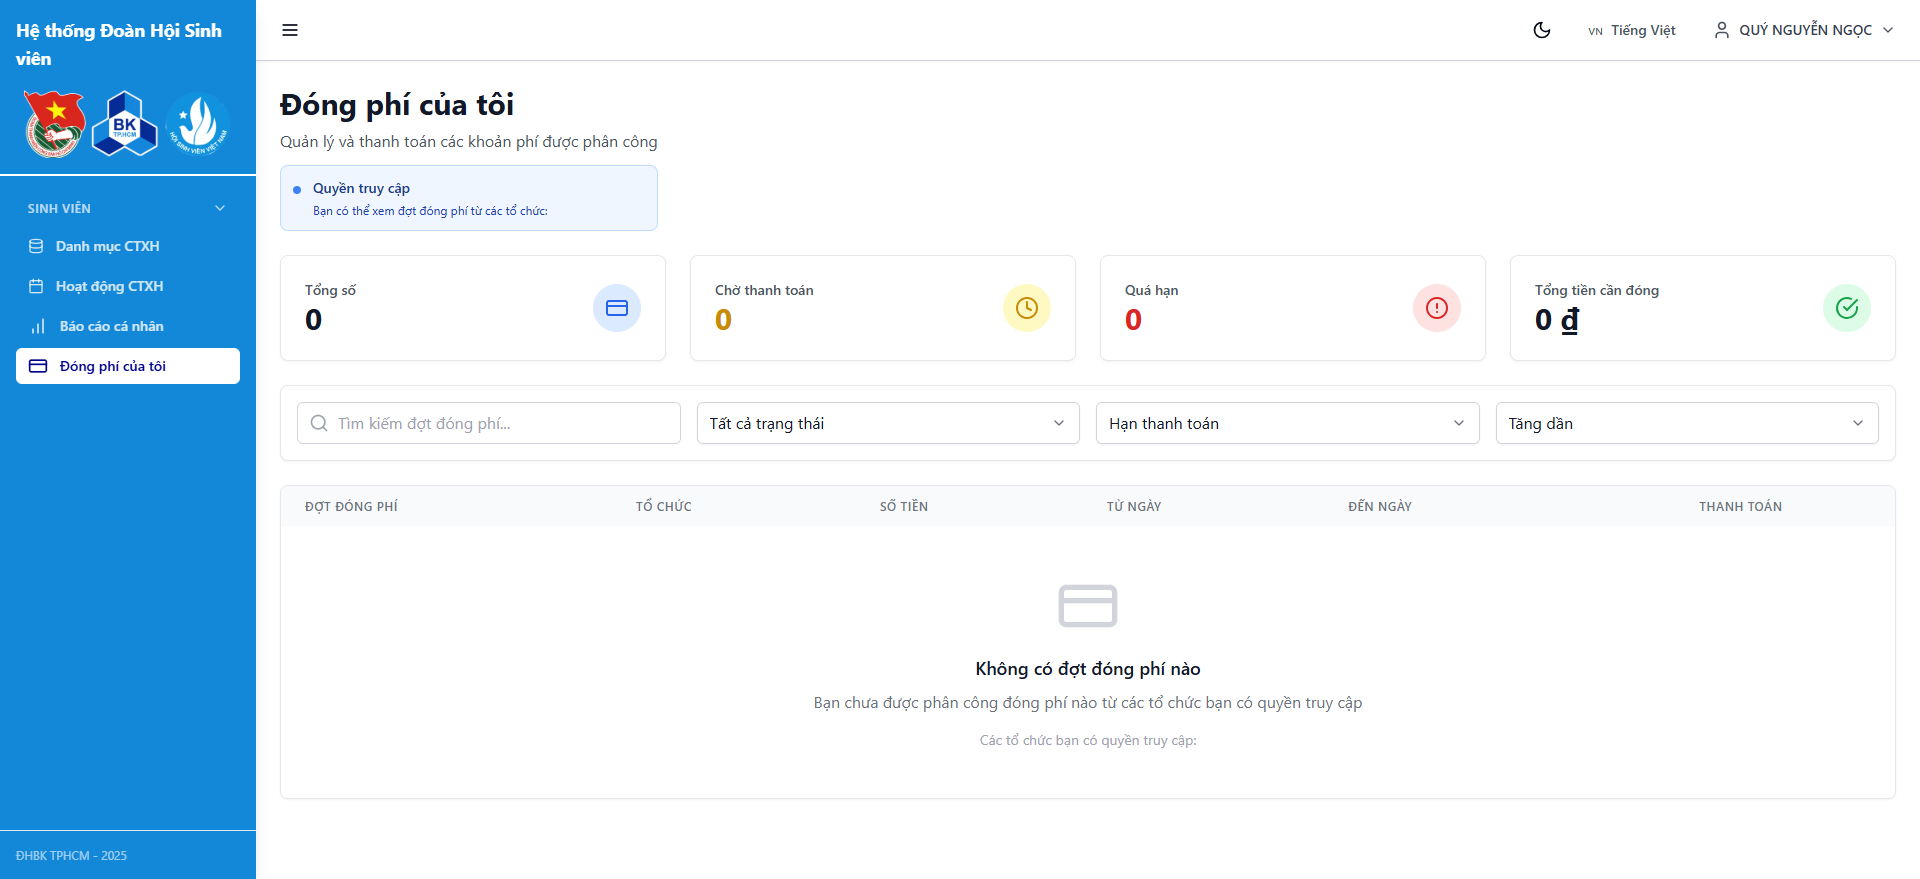
\includegraphics[width=0.96\linewidth]{Images/5.2 Hình giao diện/Module Thu phí/Trang đóng phí của tôi.png}
	\caption{Giao diện đóng phí của sinh viên}
\end{figure}

\textbf{Nhóm biểu mẫu.}
\begin{figure}[H]
	\centering
	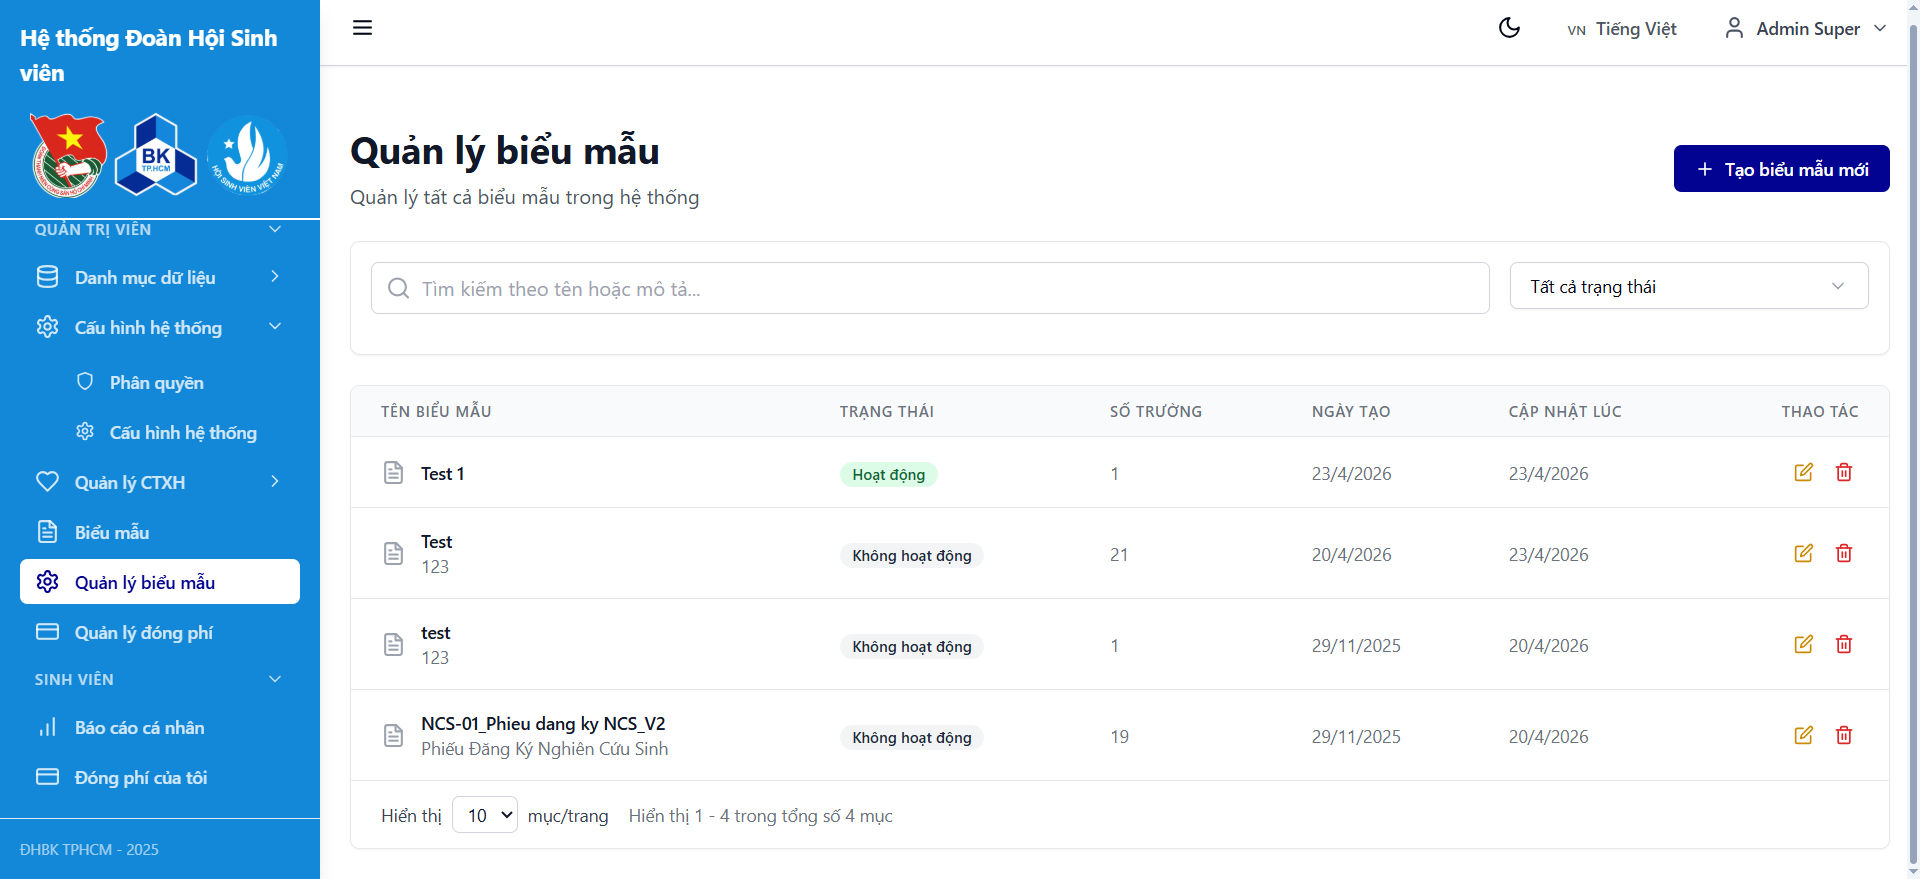
\includegraphics[width=0.96\linewidth]{Images/5.2 Hình giao diện/Trang biểu mẫu/Trang quản lý biểu mẫu.png}
	\caption{Giao diện quản lý biểu mẫu}
\end{figure}

\begin{figure}[H]
	\centering
	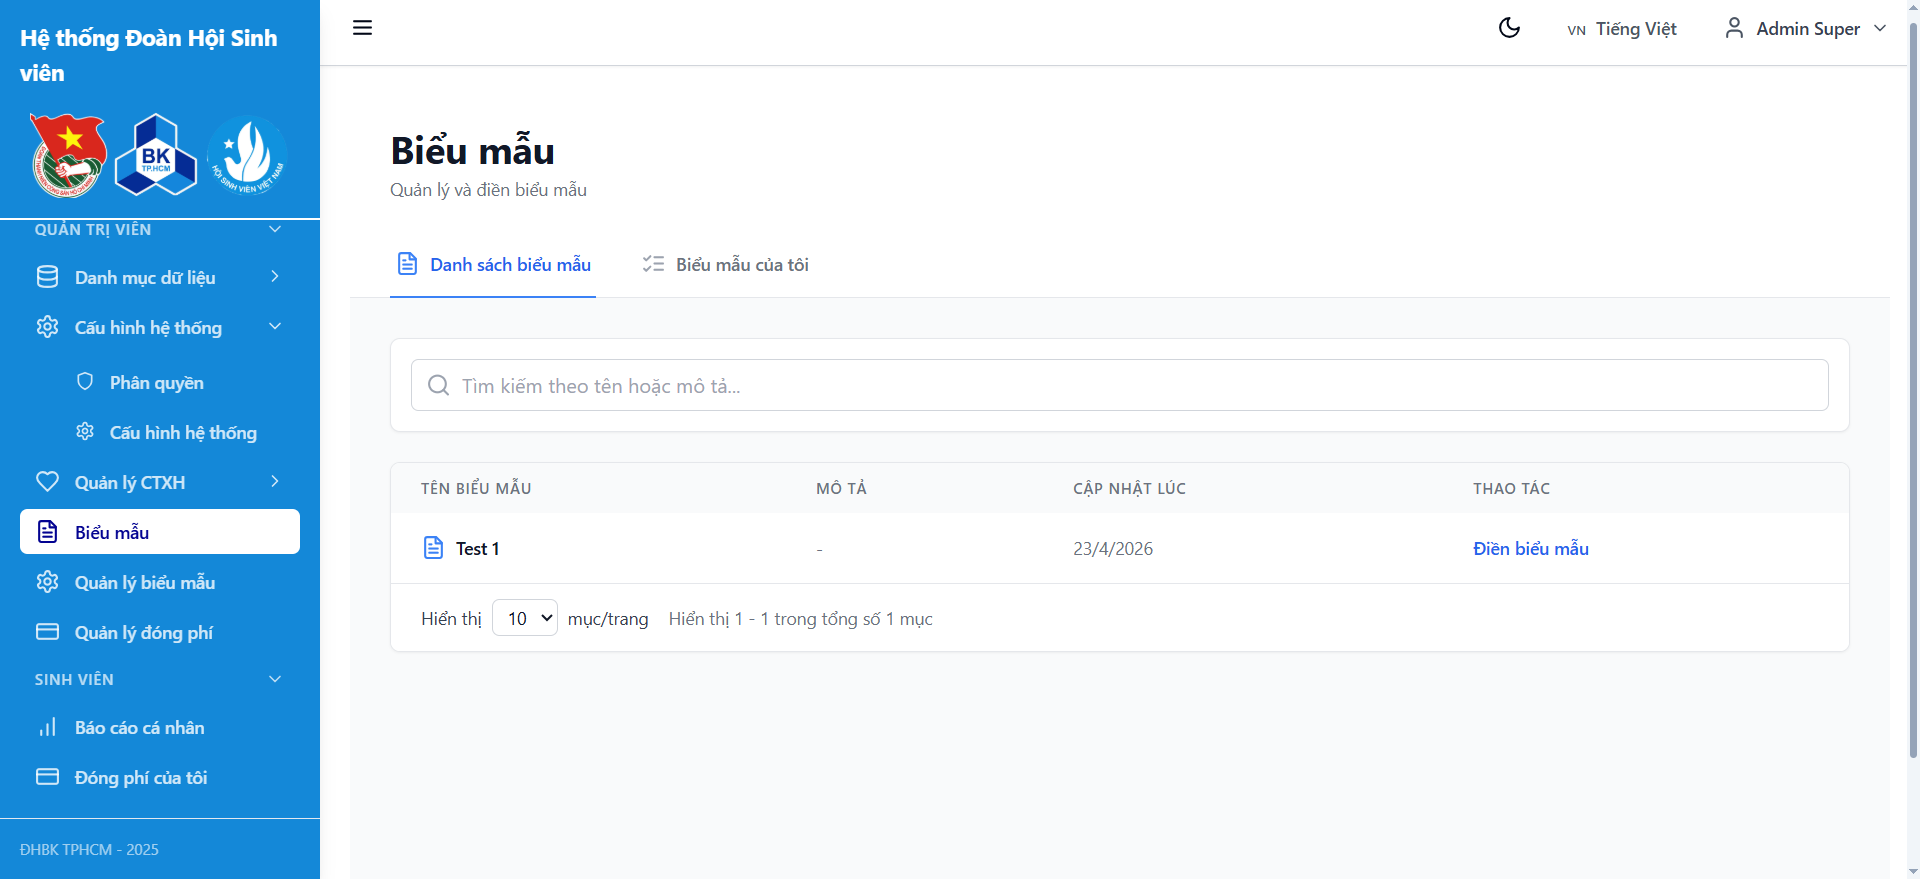
\includegraphics[width=0.96\linewidth]{Images/5.2 Hình giao diện/Trang biểu mẫu/Trang biểu mẫu - Danh sách biểu mẫu.png}
	\caption{Giao diện danh sách biểu mẫu có thể điền}
\end{figure}

\begin{figure}[H]
	\centering
	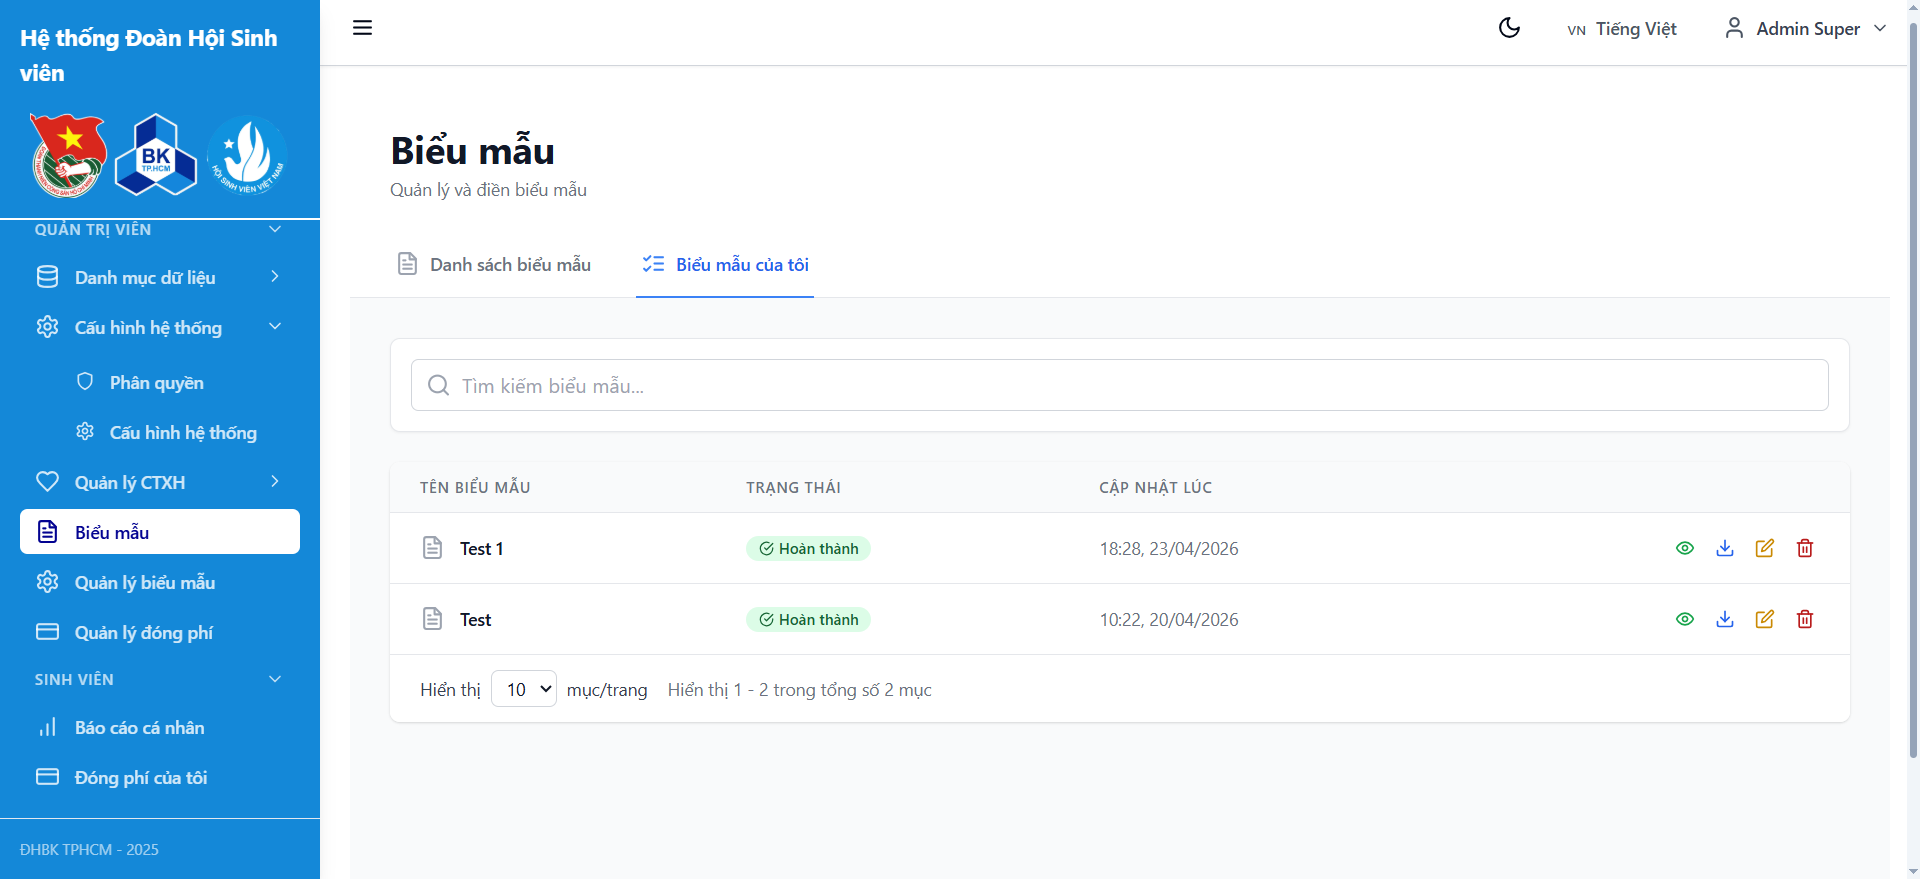
\includegraphics[width=0.96\linewidth]{Images/5.2 Hình giao diện/Trang biểu mẫu/Trang biểu mẫu - Biểu mẫu của tôi.png}
	\caption{Giao diện theo dõi biểu mẫu của tôi}
\end{figure}

\textbf{Nhóm chatbot.}
\begin{figure}[H]
	\centering
	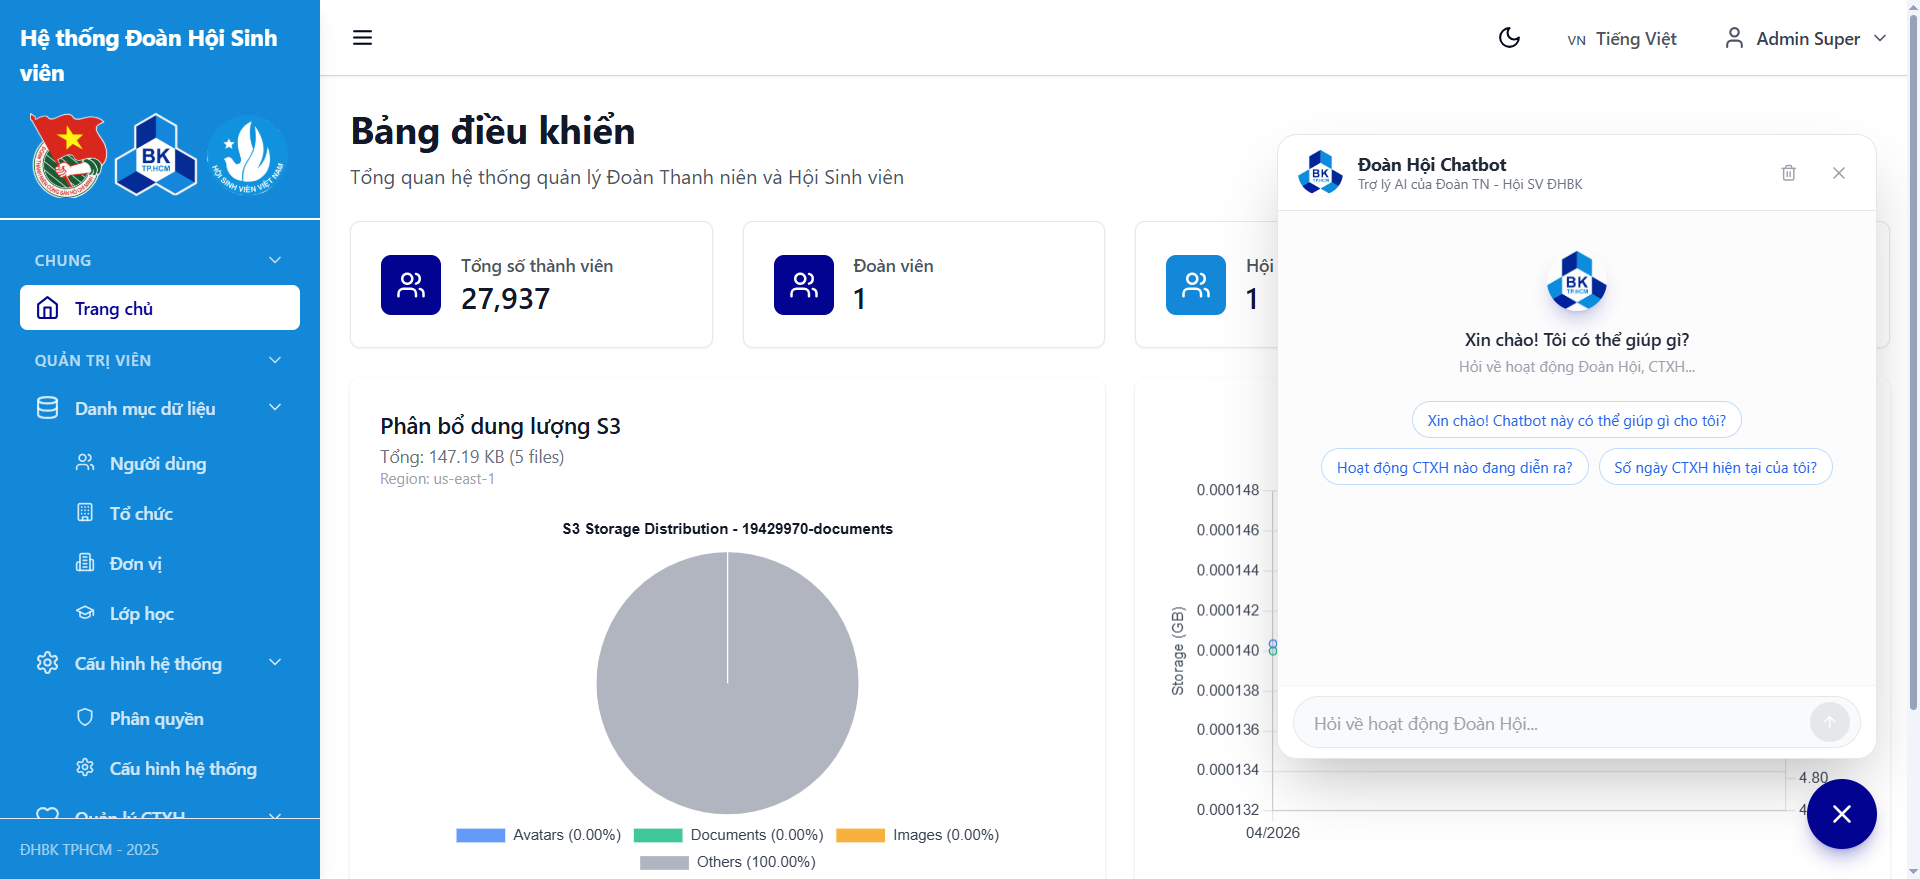
\includegraphics[width=0.96\linewidth]{Images/5.2 Hình giao diện/Chat bot RAG.png}
	\caption{Giao diện hội thoại chatbot CTXH}
\end{figure}

\begin{figure}[H]
	\centering
	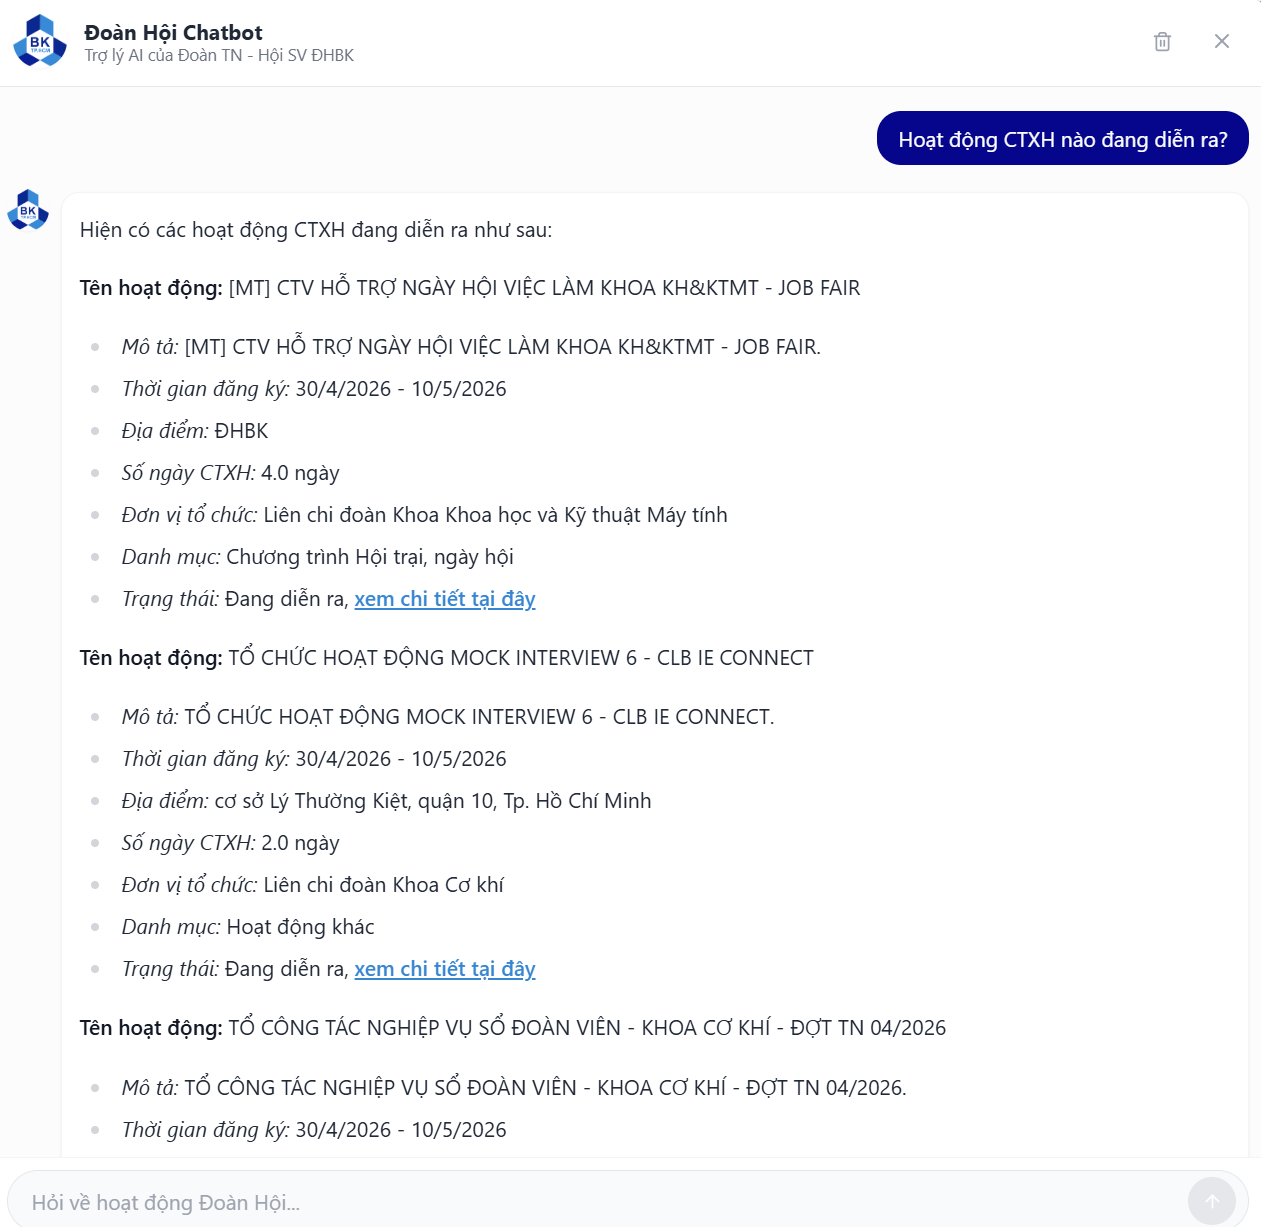
\includegraphics[width=0.96\linewidth]{Images/5.2 Hình giao diện/Chatbot_answer.png}
	\caption{Giao diện hiển thị câu trả lời từ chatbot CTXH}
\end{figure}

\begin{figure}[H]
	\centering
	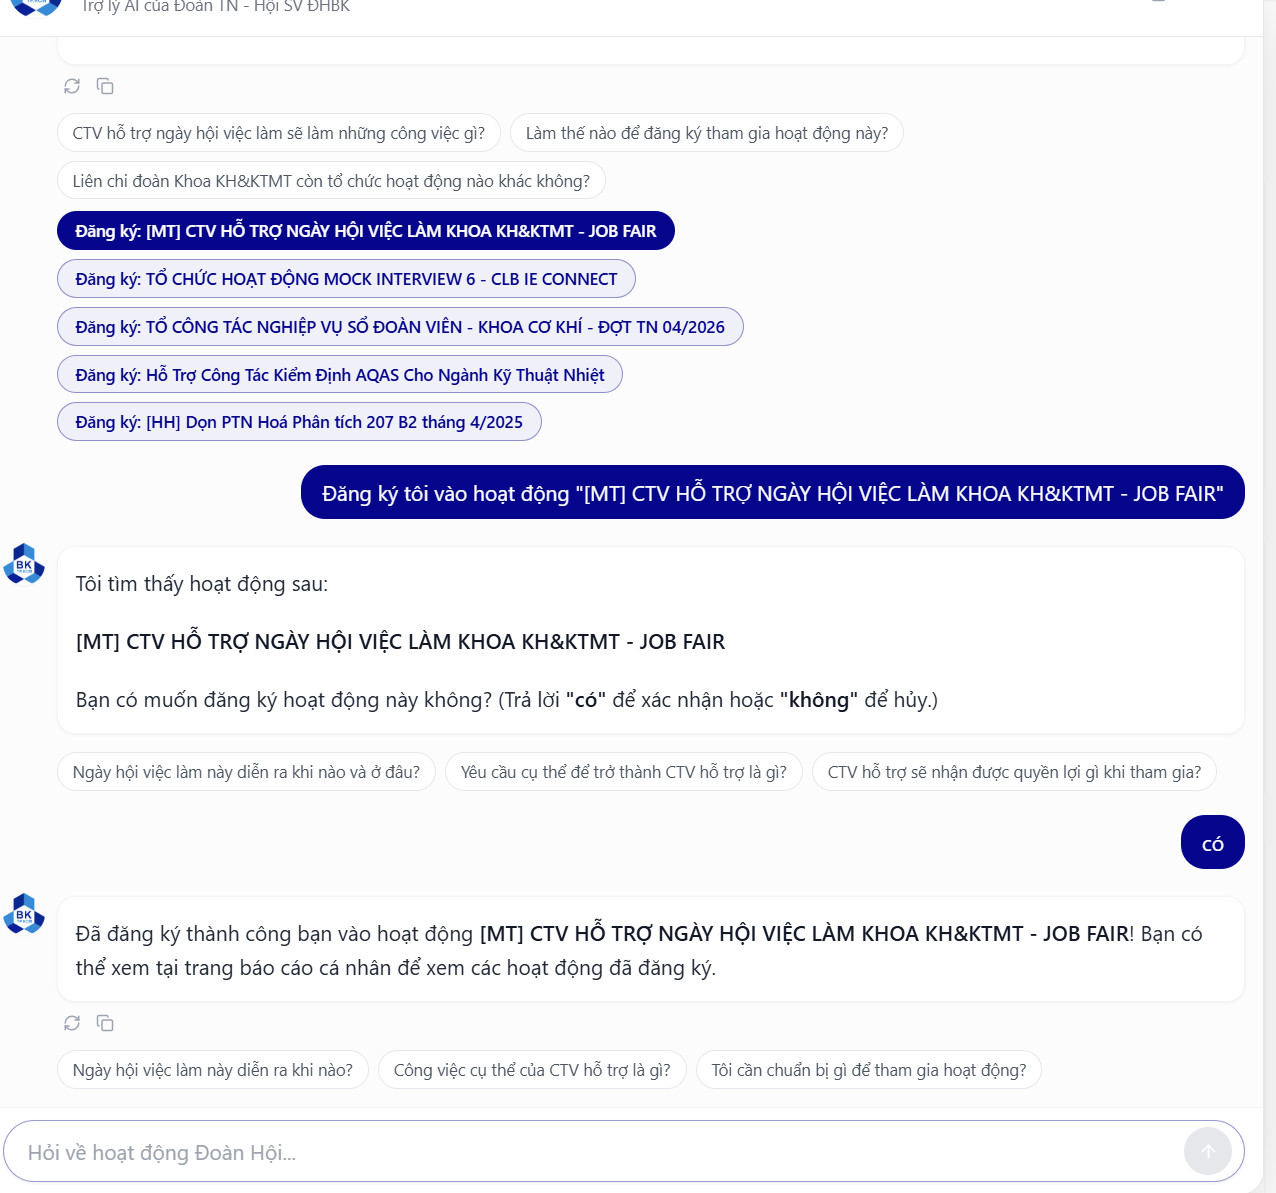
\includegraphics[width=0.96\linewidth]{Images/5.2 Hình giao diện/Chatbot_register.png}
	\caption{Giao diện đăng ký hoạt động CTXH qua chatbot}
\end{figure}

\subsubsection{Hiện thực trải nghiệm cho tác vụ dữ liệu lớn}
Các tác vụ nghiệp vụ có dữ liệu lớn được hiện thực với cơ chế giảm tải ở UI:
\begin{itemize}
	\item Phân trang và tìm kiếm phía server cho danh sách lớn.
	\item Import theo batch kèm tiến trình và tổng kết lỗi.
	\item Caching truy vấn bằng React Query để hạn chế gọi API lặp.
	\item Các màn hình cây tổ chức dùng chiến lược lazy loading để giảm tải dữ liệu ban đầu.
\end{itemize}

\subsubsection{Kết nối giữa giao diện và backend}
Mỗi màn hình frontend được gắn với tập API rõ ràng theo module. Cách tổ chức này giúp truy vết lỗi nhanh theo chiều dọc (UI $\rightarrow$ API $\rightarrow$ Service $\rightarrow$ DB) và thuận lợi khi bảo trì theo từng miền nghiệp vụ.

Về mặt vận hành, giao diện được đóng gói build tĩnh và phục vụ qua Nginx; backend cung cấp API qua domain chung, hỗ trợ CORS theo môi trường và đồng nhất cơ chế xác thực JWT cho toàn hệ thống.

\clearpage